\documentclass[a4paper,12pt]{scrreprt}
\usepackage[utf8]{inputenc}
\usepackage[provide=*,german]{babel}
\usepackage[T1]{fontenc}
\usepackage{amsmath}
\usepackage{amssymb}
\usepackage{amsthm}
\usepackage{mathtools}
\usepackage{geometry}
\usepackage{graphicx}
\usepackage[hidelinks]{hyperref}
\usepackage{xcolor}
\usepackage{float}
\usepackage{booktabs}
\usepackage{caption}
\usepackage{subcaption}
\usepackage{pgfplots}
\usepackage{microtype}
\usepackage{array}
\usepackage{rotating}
\usepackage{etoolbox}
\usepackage{enumitem}
\usepackage{tikz}
\usepackage{mdframed}
\usepackage{multirow}
\usepackage{longtable}
\usepackage{tabularx}
\usepackage{siunitx}
\usepackage{bm}
\usepackage{braket}
\usepackage{algorithm}
\usepackage{algpseudocode}
\usepackage{listings}
\usepackage{colortbl}

\setlist[itemize,1]{label=--}
\setlist[enumerate,1]{label=\arabic*.}

\usetikzlibrary{positioning,shapes,arrows,arrows.meta,calc,fit,backgrounds,
  decorations.pathmorphing,patterns,decorations.markings,mindmap,trees}
\pgfplotsset{compat=1.18}
\geometry{margin=2.5cm}

%-----------------------------------------------------------------------
% Gliederung: part für NF, section als Hauptebene
%-----------------------------------------------------------------------
\setcounter{secnumdepth}{3}

\RedeclareSectionCommand[beforeskip=2\baselineskip,afterskip=1\baselineskip,
  font=\Large\bfseries]{section}
\RedeclareSectionCommand[beforeskip=1\baselineskip,afterskip=0.5\baselineskip]{subsection}
\RedeclareSectionCommand[beforeskip=0.75\baselineskip,afterskip=0.25\baselineskip]{subsubsection}
\RedeclareSectionCommand[beforeskip=0.5\baselineskip,afterskip=-1em,
  font=\normalfont\bfseries]{paragraph}

\DeclareTOCStyleEntry[indent=0pt,numwidth=2em,entryformat=\bfseries,
  pagenumberformat=\bfseries,beforeskip=0.5em]{tocline}{section}

%-----------------------------------------------------------------------
% Theorem-Umgebungen
%-----------------------------------------------------------------------
\theoremstyle{definition}
\newtheorem{definition}{Definition}[section]
\newtheorem{satz}{Satz}[section]
\newtheorem{lemma}{Lemma}[section]
\newtheorem{korollar}{Korollar}[section]
\newtheorem{bemerkung}{Bemerkung}[section]
\newtheorem{beispiel}{Beispiel}[section]
\newtheorem{proposition}{Proposition}[section]
\newtheorem{hypothese}{Hypothese}[section]
\newtheorem{these}{These}[section]

\counterwithout{section}{chapter}
\counterwithin{figure}{section}
\counterwithin{table}{section}
\counterwithout{equation}{chapter}

\hypersetup{colorlinks=true,linkcolor=blue!60!black,urlcolor=blue!60!black,
  citecolor=blue!60!black}

%-----------------------------------------------------------------------
% Infobox
%-----------------------------------------------------------------------
\mdfdefinestyle{infobox}{linecolor=blue!50,backgroundcolor=blue!4,linewidth=1pt,
  leftline=true,rightline=false,topline=false,bottomline=false,
  innerleftmargin=12pt,innerrightmargin=10pt,innertopmargin=8pt,
  innerbottommargin=8pt,skipabove=\baselineskip,skipbelow=\baselineskip}
\newmdenv[style=infobox]{infobox}

%-----------------------------------------------------------------------
% Listings
%-----------------------------------------------------------------------
\lstset{basicstyle=\ttfamily\footnotesize,breaklines=true,frame=single,
  numbers=left,numberstyle=\tiny\color{gray},keywordstyle=\color{blue}\bfseries,
  commentstyle=\color{green!60!black},stringstyle=\color{red},
  showstringspaces=false,tabsize=4,
  literate={ä}{{\"a}}1{ö}{{\"o}}1{ü}{{\"u}}1
           {Ä}{{\"A}}1{Ö}{{\"O}}1{Ü}{{\"U}}1{ß}{{\ss}}1}

%-----------------------------------------------------------------------
% Makros
%-----------------------------------------------------------------------
\newcommand{\kb}{k_\mathrm{B}}
\newcommand{\neff}{n_\mathrm{eff}}
\newcommand{\ordre}[1]{\mathcal{O}\!\left(#1\right)}
\newcommand{\Tr}{\operatorname{Tr}}
\newcommand{\vect}[1]{\bm{#1}}
\newcommand{\matr}[1]{\mathbf{#1}}

\pretocmd{\part}{\clearpage}{}{}
\makeatletter
\@addtoreset{section}{part}
\makeatother

%=======================================================================
\title{\textbf{Neue Forschungsfelder der Naturwissenschaften}\\[0.8ex]
  \large Acht vollständige wissenschaftliche Arbeiten\\
  aus der transdisziplinären Kreuzanalyse}
\author{Stephan Epp}
\date{3. März 2026}

\begin{document}
\maketitle
\newpage

%-----------------------------------------------------------------------
\begin{center}
\Large\textbf{Vorwort}
\end{center}
\bigskip
Dieses Dokument enthält acht eigenständige wissenschaftliche Arbeiten,
die aus der systematischen Kreuzanalyse von fünfzehn Repositorien
entstanden sind. Jede Arbeit adressiert ein neues Forschungsfeld (NF-1
bis NF-8), das weder in den Einzelarbeiten noch in der bestehenden
Forschungsliteratur explizit behandelt wird.

\medskip
\begin{center}
\begin{tabular}{ll}
\toprule
\textbf{Teil} & \textbf{Forschungsfeld} \\
\midrule
NF-1 & Universelle Strukturkodierungstheorie (USK) \\
NF-2 & Hydro-ionisch-photonische Nanoplattformen (HIPN) \\
NF-3 & Post-NP-Kryptographie \\
NF-4 & Polynomielle Systembiologie \\
NF-5 & Rheoinformatik \\
NF-6 & Biomimetische Kochlea-Architektur \\
NF-7 & Ionotronische Roboter-Neuromorphie \\
NF-8 & Strukturelle Software-Graphentheorie \\
\bottomrule
\end{tabular}
\end{center}

\newpage
\tableofcontents
\newpage

%%======================================================================
%%======================================================================
\part{NF-1 \quad Universelle Strukturkodierungstheorie (USK)}
\label{part:nf1}
%%======================================================================
%%======================================================================

%=======================================================================
\section{Einleitung zur USK}
%=======================================================================

\subsection{Ausgangsfrage}

In scheinbar weit voneinander entfernten wissenschaftlichen Disziplinen
tauchen erstaunlich ähnliche mathematische Strukturen auf. Die
\textbf{Signaturfunktion} aus der Graphentheorie kodiert Spaltenvektoren
binärer Matrizen injektiv in natürliche Zahlen. Die
\textbf{Fourier-Transformation} kodiert zeitabhängige Signale in
Frequenzspektren. Die \textbf{Rotationsabbildung} überführt Wendepunkte
einer Kurve in Extrema des rotierten Bildes. Die
\textbf{Transfermatrix} propagiert elektromagnetische Felder durch
geschichtete Medien. Oberfläche: vier verschiedene Methoden in vier
Feldern. Struktur: alle vier sind \emph{injektive, strukturerhaltende
Abbildungen}.

Die \textbf{Universelle Strukturkodierungstheorie (USK)} beschreibt alle
vier als Instanzen eines gemeinsamen algebraischen Rahmens.

\subsection{Ãœberblick}

Abschnitt~\ref{sec:nf1_vier} stellt die vier Abbildungen vor.
Abschnitt~\ref{sec:nf1_rahmen} entwickelt den gemeinsamen Rahmen.
Abschnitt~\ref{sec:nf1_saetze} beweist die Hauptsätze.
Abschnitt~\ref{sec:nf1_anwendungen} zeigt Anwendungen.

%=======================================================================
\section{Die vier Kodierungsabbildungen}
\label{sec:nf1_vier}
%=======================================================================

\subsection{Signaturfunktion}

\begin{definition}[Signaturfunktion]
  Sei $A \in \{0,1\}^{n \times n}$ und $j \in \{0,\ldots,n-1\}$. Die
  \textbf{Signaturfunktion} ist
  \[
    \sigma(A, j) = \underbrace{\sum_{i=0}^{n-1} A_{ij} \cdot 2^i}_{\rho(A,j)}
    + \underbrace{j \cdot 2^n}_{\lambda(j)}.
  \]
\end{definition}

Sie ist injektiv: verschiedene $(A,j)$ liefern verschiedene Werte.
Erhaltene Struktur: die \emph{Subgraph-Relation}.

\begin{lemma}[Strukturerhaltung $\sigma$]
  $G \subseteq G' \implies \mathrm{LCS}(\rho(A),\rho(B)) \geq 2.$
\end{lemma}

\subsection{Fourier-Transformation}

\begin{definition}[Fourier-Transformation]
  \[
    \hat{f}(\xi) = \int_{-\infty}^{+\infty} f(t)\,e^{-2\pi i\xi t}\,dt,
    \quad f \in L^2(\mathbb{R}).
  \]
\end{definition}

Unitäre Abbildung auf $L^2$ (Plancherel: $\|\hat f\|_2 = \|f\|_2$).
Erhaltene Struktur: \emph{Signalenergie}.

\subsection{Rotationsabbildung}

\begin{definition}[Rotation]
  $R_\varphi \begin{pmatrix}x\\y\end{pmatrix}
  = \begin{pmatrix}\cos\varphi & -\sin\varphi\\\sin\varphi &
  \cos\varphi\end{pmatrix}\begin{pmatrix}x\\y\end{pmatrix}.$
\end{definition}

Operiert auf Graphen $\Gamma_f$; überführt Wendepunkte in Extrema.
Erhaltene Struktur: \emph{analytische Ordnung der Kurve}.

\subsection{Transfermatrix}

\begin{definition}[Transfermatrix]
  Für eine dielektrische Schicht mit optischer Dicke $\delta_k$:
  \[
    M_k = \begin{pmatrix}
      \cos\delta_k & -\tfrac{i}{\eta_k}\sin\delta_k \\
      -i\eta_k\sin\delta_k & \cos\delta_k
    \end{pmatrix}, \quad \eta_k = n_k\cos\theta_k.
  \]
  Systemmatrix: $M = M_N \cdots M_1 \in \mathrm{SL}(2,\mathbb{C})$.
\end{definition}

Erhaltene Struktur: \emph{Energie-Flussdichte} (Poynting-Invarianz,
$\det M = 1$).

%=======================================================================
\section{Gemeinsamer algebraischer Rahmen}
\label{sec:nf1_rahmen}
%=======================================================================

\begin{definition}[Strukturkodierungs-Paar]
  Ein \textbf{Strukturkodierungs-Paar} $(S, K, \kappa, \mathcal{P})$
  besteht aus Strukturraum $S$, Kodierungsraum $K$,
  Abbildung $\kappa: S \to K$ und Relation $\mathcal{P}$.
  Es heißt \textbf{strukturerhaltend}, wenn
  $(s_1,s_2)\in\mathcal{P} \Rightarrow (\kappa(s_1),\kappa(s_2))\in\mathcal{P}_K$.
\end{definition}

\begin{satz}[Universelles Klassifikationstheorem]
  \label{satz:nf1_usk}
  Die vier Paare sind strukturerhaltend:

  \smallskip
  \begin{center}\small
  \begin{tabular}{lllll}
  \toprule
  & $S$ & $K$ & $\kappa$ & $\mathcal{P}$ \\
  \midrule
  $\sigma$ & $\{0,1\}^{n\times n}$ & $\mathbb{N}$ & Signatur & Subgraph $\subseteq$ \\
  $\mathcal{F}$ & $L^2(\mathbb{R})$ & $L^2(\mathbb{R})$ & Fourier & Energiegleich. \\
  $R_\varphi$ & $C^2$-Kurven & $\mathrm{SO}(2)$-Orbit & Rotation & Analyt. Ordnung \\
  $M$ & Felder $\Psi$ & $\mathrm{SL}(2,\mathbb{C})$ & Transfermatrix & Flusserhaltung \\
  \bottomrule
  \end{tabular}
  \end{center}
\end{satz}

\begin{definition}[WFSE-Algebra]
  Eine \textbf{Winkel-Frequenz-Signatur-Einheit (WFSE)} ist ein Quadrupel
  $(\mathcal{A}, \cdot, *, \|\cdot\|)$ mit sequentieller Komposition
  $\cdot$, paralleler Ãœberlagerung $*$ und einer Invarianznorm
  $\|\cdot\|$, sodass
  $\|\kappa_1 \cdot \kappa_2\| = \|\kappa_1\|\cdot\|\kappa_2\|$.
\end{definition}

\begin{satz}[WFSE-Konsistenz]
  Die vier Kompositionsregeln übersetzen die strukturelle Komposition
  in algebraische Produkte:
  \begin{align*}
    R_\varphi \cdot R_\psi &= R_{\varphi+\psi}, \\
    M(z_N,z_0) &= M(z_N,z_{N-1})\cdots M(z_1,z_0), \\
    \mathcal{F}\{f*g\} &= \hat f \cdot \hat g, \\
    \sigma(A\wedge B,j) &= \sigma(A,j)\;\&\;\sigma(B,j).
  \end{align*}
\end{satz}

%=======================================================================
\section{Hauptsätze der USK}
\label{sec:nf1_saetze}
%=======================================================================

\begin{satz}[Kontinuumsgrenzwert der Signatur]
  Für den Binärvektor $v\in\{0,1\}^n$ und die Treppenfunktion
  $f_v:[0,1]\to\{0,1\}$ gilt
  \[
    \lim_{n\to\infty}\frac{\sigma(v)}{2^n} = \int_0^1 f_v(t)\,dt = \|f_v\|_{L^1}.
  \]
  Die Signaturfunktion ist das \emph{diskrete Analogon} der Fourier-Transformation.
\end{satz}

\begin{satz}[TMM-Rotations-Isomorphie]
  Jede Schicht-Transfermatrix $M_k$ mit reellen $n_k$ ist formal isomorph
  zu einer Block-Rotation mit Phase $\delta_k$. Im Grenzfall
  $n_k\to 1$ degeneriert $M_k$ zur reinen Phasenrotation $e^{i\delta_k}$.
  Die TMM ist damit eine Verallgemeinerung von $R_\varphi$ auf
  $\mathrm{SL}(2,\mathbb{C})$.
\end{satz}

\begin{infobox}
\textbf{USK-Hierarchie:}
$\sigma \subset \mathrm{DFT} \subset \mathcal{F} \supset R_\varphi \subset M_k \subset U(t)$ \\
(diskret $\to$ komplex $\to$ unitär $\to$ quantenmechanisch)
\end{infobox}

%=======================================================================
\section{Anwendungen der USK}
\label{sec:nf1_anwendungen}
%=======================================================================

\paragraph{FFT-Subgraph.} Das LCS-Kriterium des Subgraph Algorithmus wird
durch FFT-Kreuzkorrelation ersetzt. Laufzeit: $O(n^2 \log n)$ statt
$O(n^3)$.

\paragraph{TMM-Kompression.} Adjazenzmatrizen großer Graphen ($n>10^4$)
werden als photonische Schichtsysteme dargestellt; die $2\times 2$-Transfermatrix
komprimiert die gesamte Strukturinformation.

\paragraph{Geometrischer Feature-Detektor.} Die Rotationsmethode wird
auf $d$-dimensionale Datenwolken verallgemeinert: Eine Folge
$R_{\varphi_1},R_{\varphi_2},\ldots$ macht Häufungspunkte und Trennflächen
als Extrema sichtbar --- ein neues Konzept für Geometric Deep Learning.

%%======================================================================
%%======================================================================
\part{NF-2 \quad Hydro-ionisch-photonische Nanoplattformen (HIPN)}
\label{part:nf2}
%%======================================================================
%%======================================================================

%=======================================================================
\section{Einleitung zur HIPN}
%=======================================================================

\subsection{Drei komplementäre Technologiestränge}

Das \textbf{Ionotronic Reconfigurable Fabric} (IRF) nutzt ionisch
dotiertes Wasser als simultanen Leiter, Schalter und Speicher. Die
\textbf{aktive Nanooptik} stimmt Fabry-Pérot-Polymer-Resonatoren durch
Quellung im Bereich \SIrange{420}{700}{nm}. Die \textbf{Viskoelastizität
hydraulischer Öle} überträgt mechanische Kräfte mit einem Bulkmodul
$K \approx \SI{1.7}{GPa}$.

Die \textbf{Hydro-ionisch-photonische Nanoplattform (HIPN)} vereint
alle drei Stränge zu einem \emph{tri-funktionalen} System: Rechnen,
Anzeigen, Aktuieren in einer einzigen Flüssigkeits-Polymer-Struktur.

\begin{infobox}
\textbf{HIPN-Triplexitätsprinzip.} Das Flüssigkeitssystem (Wasser +
ionische Additive + Polymer) übernimmt gleichzeitig
\textbf{Berechnung} (IoFET), \textbf{Anzeige} (Strukturfarbe) und
\textbf{Aktuierung} (Hydraulik).
\end{infobox}

%=======================================================================
\section{Physikalische Grundlagen der Triplexität}
%=======================================================================

\subsection{Computerschicht: IoFET und EWOD}

Die Lippmann-Young-Gleichung für das Kontaktwinkeln eines Tropfens
unter Spannung $V$:
\[
  \cos\theta(V) = \cos\theta_0 + \frac{\varepsilon_0\varepsilon_r}{2\gamma_{LG}d}\,V^2.
\]
Durch Modulieren von $V$ an benachbarten ITO-Elektroden werden Tropfen
geleitet, gespalten, zusammengeführt -- Tropfenlogik.

\subsection{Anzeigeschicht: Fabry-Pérot-Quellung}

Resonanzwellenlänge eines Polymer-Resonators der Dicke $d$:
$\lambda_m = 2nd/m$. Das Flory-Rehner-Quellungsgesetz ergibt
\[
  \ln(1-\phi_p)+\phi_p+\chi\phi_p^2
  + V_1\nu\bigl(\phi_p^{1/3}-\tfrac{\phi_p}{2}\bigr)=0.
\]
Durch IoFET-gesteuerte lokale Wasserkonzentration wird $\phi_p(x,y,t)$
und damit $\lambda_m$ pixelgenau eingestellt.

\subsection{Aktuierungsschicht: Hydraulische Elastizität}

Bulkmodul mit Druckabhängigkeit: $K(p) = K_0 + \alpha p$,
$\alpha \approx 6$--$10$. Maximale Schaltfrequenz:
\[
  f_{\max} = \frac{\sqrt{K/\rho}}{2L} \approx \SI{22}{kHz}
  \text{ für } L=\SI{10}{mm}.
\]

%=======================================================================
\section{HIPN-Architektur und Hydrokanal-SAT}
%=======================================================================

\subsection{Schichtaufbau}

Der vertikale Aufbau von oben nach unten:
\begin{itemize}
  \item \textbf{IoFET-Computerschicht}: KCl-Lösung, Parylene-C-Dielektrikum,
    ITO-Elektroden (\SI{10}{\micro m} Pitch).
  \item \textbf{Polymer-Anzeigeschicht}: PDMS-Hydrogel (\SI{150}{nm}),
    TiO\textsubscript{2}/SiO\textsubscript{2}-Bragg-Spiegel.
  \item \textbf{Hydraulische Aktuierungsschicht}: Mineralöl ISO VG 46,
    piezoelektrische Mikropumpe, Kapton-Membran.
\end{itemize}
Kopplung: Computerschicht steuert Wasserzufuhr $\to$ Anzeigeschicht
ändert $\phi_p$ $\to$ Laplace-Druck $\Delta p = \gamma_{LG}\kappa_c$
wirkt auf Aktuierungsschicht.

\subsection{Hydrokanal-SAT}

\begin{satz}[Hydrokanal-SAT-Korrektheit]
  Eine 3-CNF-Formel $\Phi$ über $n$ Variablen und $m$ Klauseln wird als
  Tropfenflussnetzwerk der Größe $O(n+m)$ kodiert. Die Formel ist
  satisfizierbar genau dann, wenn alle $m$ Klausel-Sammelkanäle Fluss
  führen. Die physikalische Rechenzeit ist $\tau = L/v_{\mathrm{drop}}$.
\end{satz}

\subsection{Leistungsparameter}

\begin{table}[H]
\small
\caption{HIPN vs.\ CMOS \SI{3}{nm}}
\label{tab:nf2_vergleich}
\begin{tabular}{lll}
\toprule
\textbf{Parameter} & \textbf{CMOS 3 nm} & \textbf{HIPN} \\
\midrule
Schaltenergie       & $<\SI{1}{aJ}$      & $\sim\SI{1}{pJ}$ \\
Schaltzeit          & $<\SI{1}{ps}$      & $<\SI{1}{ms}$ \\
Funktionen/Einheit  & 1                  & \textbf{3} (Rechnen+Anzeigen+Aktuieren) \\
Kühlung nötig       & Ja                 & Nein \\
Selbstheilend       & Nein               & Ja \\
Lithographie nötig  & Ja                 & Nein \\
\bottomrule
\end{tabular}
\end{table}

%=======================================================================
\section{Anwendungen der HIPN}
%=======================================================================

\paragraph{Retina-Implantat.} $256\times 256$ IoFET-Matrix auf
\SI{4}{mm^2}: Bildsignal $\to$ Strukturfarbe $\to$ Druckpulse zur
Ganglienzellen-Stimulation.

\paragraph{Adaptive Tarnung.} \SI{10}{cm^2}-Panel mit \SI{100}{\micro m}/Pixel,
Farbwechsel $<\SI{200}{ms}$ -- identisch mit Oktopus-Biologie.

\paragraph{Lab-on-Chip.} Biochemische SAT-Probleme (PCR-Primer-Design,
Protein-Bindung) als physikalische Tropfenfluss-Berechnung auf dem
HIPN-Chip.

%%======================================================================
%%======================================================================
\part{NF-3 \quad Post-NP-Kryptographie}
\label{part:nf3}
%%======================================================================
%%======================================================================

%=======================================================================
\section{Einleitung zur Post-NP-Kryptographie}
%=======================================================================

\subsection{Die neue kryptographische Lage nach P=NP}

Der Beweis P=NP durch den Subgraph Algorithmus $O(n^3)$ hat eine
fundamentale Konsequenz: \emph{Alle Kryptosysteme, deren Sicherheit auf
der Unlösbarkeit NP-schwerer Probleme beruht, sind gebrochen.}

\begin{itemize}
  \item \textbf{RSA} gebrochen: Faktorisierung ist polynomiell lösbar.
  \item \textbf{ECDH, ECDSA, Ed25519} gebrochen: Diskreter Logarithmus
    auf elliptischen Kurven (ECDLP) ist polynomiell.
  \item \textbf{Diffie-Hellman} gebrochen: Diskreter Logarithmus mod $p$
    polynomiell.
  \item \textbf{LWE/NTRU (Post-Quantum-Kandidaten)} gebrochen:
    Gitterprobleme (SVP, CVP) sind NP-hart und damit polynomiell.
  \item \textbf{McEliece} gebrochen: Code-Decodierung (NP-vollständig)
    polynomiell.
\end{itemize}

Nicht gebrochen:
\begin{itemize}
  \item \textbf{AES}: Sicherheit beruht auf algebraischer Resistenz, nicht
    auf NP-Schwierigkeit.
  \item \textbf{SHA-256}: Einwegfunktion durch Diffusion/Konfusion.
  \item \textbf{One-Time-Pad}: Informationstheoretisch-perfekte Sicherheit
    (Shannon 1949).
\end{itemize}

\subsection{Ziel dieser Arbeit}

Systematische Neuordnung der Kryptographie nach P=NP:
(\textit{i})~Klassifizierung gebrochener und resistenter Verfahren,
(\textit{ii})~Formalisierung der Signatur-Chiffre als neues Paradigma,
(\textit{iii})~ionotronische Schlüsselerzeugung als physikalische
Entropiequelle.

%=======================================================================
\section{Mathematische Grundlagen}
%=======================================================================

\subsection{Die Signaturfunktion als kryptographisches Primitiv}

\begin{definition}[Signaturfunktion, kryptographische Version]
  Sei $A \in \{0,1\}^{n\times n}$, $j\in\{0,\ldots,n-1\}$. Die
  Signaturfunktion ist
  $\sigma(A,j) = \sum_{i=0}^{n-1} A_{ij} \cdot 2^i + j \cdot 2^n.$
  Sie ist injektiv: $\sigma(A,j) = \sigma(A',j') \Rightarrow
  j=j'$ und $A_{\cdot j} = A'_{\cdot j'}$.
\end{definition}

\subsection{Der geheime Primzahlkörper}

\begin{definition}[Primzahlkörper $\mathbb{Z}_p$]
  Sei $p$ eine Primzahl. Der Körper $\mathbb{Z}_p = \{0,1,\ldots,p-1\}$
  mit Addition und Multiplikation modulo $p$ ist ein endlicher Körper
  mit $p$ Elementen. Für $p$ eine 256-Bit-Primzahl hat $\mathbb{Z}_p$
  ca.\ $2^{256}$ Elemente.
\end{definition}

\subsection{Affine Transformation als Baustein}

Die affine Chiffre über $\mathbb{Z}_{26}$ mit optimalen Parametern
$a=15$, $b=29$ ($\equiv 3 \bmod 26$) zeigt das Grundprinzip:
$E(x) = (ax+b)\bmod m$,\; $D(y) = a^{-1}(y-b)\bmod m$.
Die Signatur-Chiffre überträgt dieses Prinzip auf den geheimen
Primzahlkörper $\mathbb{Z}_p$ mit einer 256-Bit-Primzahl $p$.

%=======================================================================
\section{Die Signatur-Chiffre}
%=======================================================================

\subsection{Konstruktion}

\begin{definition}[Signatur-Chiffre]
  Sei $p$ eine geheime 256-Bit-Primzahl, $a,b\in\mathbb{Z}_p^*$ mit
  $\gcd(a,p)=1$. Für einen Klartextblock $X \in \{0,1\}^{n\times n}$
  ist die \textbf{Signatur-Chiffre} definiert als:
  \begin{align*}
    \text{Verschlüsselung:} &\quad c_j = (a \cdot \sigma(X,j) + b) \bmod p \\
    \text{Entschlüsselung:} &\quad \sigma(X,j) = a^{-1}(c_j - b) \bmod p
  \end{align*}
  Der Schlüssel ist das Tripel $(p, a, b)$.
\end{definition}

\begin{satz}[Korrektheit]
  Sei $c_j$ das Chiffrat von $\sigma(X,j)$ unter $(p,a,b)$. Dann gilt
  $D(c_j) = a^{-1}(c_j-b)\bmod p = \sigma(X,j)$. Da $\sigma$ injektiv
  ist, ist $X$ eindeutig rekonstruierbar.
\end{satz}

\begin{proof}
  $D(c_j) = a^{-1}((a\sigma(X,j)+b)-b)\bmod p
  = a^{-1} a \sigma(X,j)\bmod p = \sigma(X,j).$
\end{proof}

\subsection{Sicherheitsanalyse}

\begin{satz}[Äquivokation]
  Ohne Kenntnis der Primzahl $p$ ist für den Angreifer nicht einmal
  bekannt, in welchem algebraischen Körper die Entschlüsselung stattfindet.
  Der Schlüsselraum für eine 256-Bit-Primzahl $p$ umfasst ca.\ $2^{512}$
  Elemente (Wahl von $p$, $a$, $b$).
\end{satz}

\begin{satz}[Resistenz gegen Subgraph-Angriff]
  Der Subgraph Algorithmus löst das Subgraph-Isomorphismus-Problem.
  Die Signatur-Chiffre beruht jedoch nicht auf Subgraph-ISO, sondern
  auf der Unkenntnis des Primzahlkörpers $\mathbb{Z}_p$ -- einem Problem,
  das nicht auf Graphenprobleme reduzierbar ist.
\end{satz}

%=======================================================================
\section{Ionotronische Schlüsselerzeugung}
%=======================================================================

\subsection{Physikalischer Zufall im IoFET}

Das IRF-System erzeugt von Natur aus nicht-deterministisches Verhalten
durch thermisches Rauschen bei Tropfen-Kollisionen. Die
Tropfen-Kollisionszeit $\tau_c$ folgt einer Poisson-Verteilung mit
Rate $\lambda_c$. Dies liefert einen \textbf{physikalischen
Zufallsgenerator (TRNG)}.

\begin{definition}[IoFET-TRNG]
  Ein \textbf{ionotronischer True-Random-Number-Gene\-rator} misst die
  Zeitdifferenzen $\Delta t_k = \tau_{k+1} - \tau_k$ zwischen
  aufeinanderfolgenden Tropfen-Kollisions\-ereignissen und erzeugt Bits
  durch $b_k = \mathbf{1}[\Delta t_k > \bar{\tau}]$, wobei
  $\bar\tau$ der empirische Median ist.
\end{definition}

\begin{satz}[Statistische Qualität]
  Die erzeugten Bits sind unkorreliert (unabhängige Poisson-Ereignisse),
  gleichverteilt (Median-Schwellwert) und nicht reproduzierbar
  (thermisches Rauschen). Sie erfüllen die NIST-SP-800-22-Testanforderungen.
\end{satz}

\subsection{Schlüsselerzeugungsprotokoll}

\begin{enumerate}
  \item IoFET-TRNG erzeugt $512$ Zufallsbits $b_1,\ldots,b_{512}$.
  \item Die ersten 256 Bits definieren Kandidaten-Primzahl durch
    Miller-Rabin-Test.
  \item Falls nicht prim, wiederhole ab Schritt 1.
  \item $a, b \in \mathbb{Z}_p^*$ werden aus weiteren 512 TRNG-Bits
    bestimmt.
\end{enumerate}

%=======================================================================
\section{Vollständige kryptographische Landkarte nach P=NP}
%=======================================================================

\begin{longtable}{p{3.5cm}p{3cm}p{4.5cm}p{3cm}}
\caption{Kryptographische Verfahren nach P=NP}
\label{tab:nf3_krypto}\\
\toprule
\textbf{Verfahren} & \textbf{Hartes Problem} & \textbf{Status nach P=NP} & \textbf{Ersatz} \\
\midrule
\endfirsthead
\toprule
\textbf{Verfahren} & \textbf{Hartes Problem} & \textbf{Status} & \textbf{Ersatz} \\
\midrule
\endhead
\bottomrule
\endfoot
RSA-2048        & Faktorisierung    & \textcolor{red}{Gebrochen}  & Signatur-Chiffre \\
ECDH/ECDSA      & ECDLP             & \textcolor{red}{Gebrochen}  & Signatur-Chiffre \\
Diffie-Hellman  & DLP               & \textcolor{red}{Gebrochen}  & Signatur-Chiffre \\
McEliece        & Code-Decodierung  & \textcolor{red}{Gebrochen}  & Signatur-Chiffre \\
NTRU/Kyber      & SVP/CVP (Gitter)  & \textcolor{red}{Gebrochen}  & Signatur-Chiffre \\
AES-256         & Algebraisch       & \textcolor{green!60!black}{Sicher} & -- \\
SHA-256/3       & Diffusion         & \textcolor{green!60!black}{Sicher} & -- \\
One-Time-Pad    & Informationstheo. & \textcolor{green!60!black}{Sicher} & -- \\
Signatur-Chiffre & Äquivokation $\mathbb{Z}_p$ & \textcolor{green!60!black}{Sicher} & -- \\
\end{longtable}

%%======================================================================
%%======================================================================
\part{NF-4 \quad Polynomielle Systembiologie}
\label{part:nf4}
%%======================================================================
%%======================================================================

%=======================================================================
\section{Einleitung zur polynomiellen Systembiologie}
%=======================================================================

\subsection{Das Skalierungsproblem der klassischen Systembiologie}

Die klassische Systembiologie scheitert an der kombinatorischen
Explosion beim Netzwerkvergleich. Das Subgraph-Isomorphismus-Problem
ist NP-vollständig; naive Permutationsansätze haben Laufzeit $O(n!)$.
Bei biologischen Netzwerken mit 50--100 Knoten sind solche Verfahren
in der Praxis nicht nutzbar.

Mit P=NP und dem Subgraph Algorithmus $O(n^3)$ ist dieses Problem gelöst.
\textbf{Polynomielle Systembiologie} bezeichnet die konsequente
Anwendung dieser Erkenntnis auf alle Bereiche der modernen Biologie:
Genomik, Proteomik, Metabolomik, Neurowissenschaft, Pharmakologie.

%=======================================================================
\section{Biologische Netzwerke als Graphen}
%=======================================================================

\begin{definition}[Biologisches Netzwerk]
  Ein biologisches Netzwerk ist ein gerichteter Graph $G=(V,E)$ mit
  \begin{itemize}
    \item $V$ = biologische Entitäten (Metabolite, Proteine, Gene,
      Neuronen),
    \item $E \subseteq V\times V$ = biologische Interaktionen
      (Reaktionen, Bindungen, Regulation, Synapsen).
  \end{itemize}
\end{definition}

\subsection{Netzwerkklassen}

\begin{table}[H]
\caption{Biologische Netzwerkklassen und ihre Grapheigenschaften}
\label{tab:nf4_netze}
\begin{tabular}{lllll}
\toprule
\textbf{Typ} & \textbf{Knoten} & \textbf{Kanten} & \textbf{Dichte $\rho$} & \textbf{Beispiel-DB} \\
\midrule
Metabolisch    & Metabolite & Enzymat. Reaktionen & $\approx 0.05$--$0.2$ & KEGG \\
Protein-PPI    & Proteine   & Physische Bindung   & $\approx 0.01$--$0.5$ & STRING \\
Gen-Regulation & Gene       & Transkript.-Faktor  & $\approx 0.01$--$0.1$ & RegulonDB \\
Neuronal       & Neuronen   & Synapsen            & $\approx 0.001$--$0.1$ & ConnectomeDB \\
\bottomrule
\end{tabular}
\end{table}

%=======================================================================
\section{Polynomieller Netzwerkvergleich}
%=======================================================================

\subsection{Subgraph Algorithmus auf biologischen Netzwerken}

\begin{satz}[Polynomielle Netzwerkvergleich-Komplexität]
  Zwei biologische Netzwerke $G=(V,E)$ und $G'=(V',E')$ mit
  $|V|=n$, $|V'|=m$ können in $O(n^2 m)$ Zeit auf Subgraph-Relation
  geprüft werden.
\end{satz}

Die Signaturfunktion liefert Fingerabdrücke biologischer Netzwerke:
Zwei Netzwerke, die strukturell äquivalent sind (z.\ B.\ homologe
Stoffwechselwege), haben übereinstimmende Signatur-Teilsequenzen.

\subsection{Algorithmisches Framework}

\begin{algorithm}[H]
\caption{Polynomielle biologische Netzwerkanalyse}
\label{alg:nf4}
\begin{algorithmic}[1]
\Require Netzwerke $G_1, G_2, \ldots, G_k$ (z.\ B.\ KEGG-Datenbank)
\Ensure Alle Subgraph-Relationen und konservierte Motive
\For{alle Paare $(G_i, G_j)$, $i < j$}
  \State Berechne Signaturen $\Sigma(G_i)$, $\Sigma(G_j)$
  \State Prüfe LCS($\Sigma(G_i)$, $\Sigma(G_j)$) $\geq 2$
  \If{Subgraph-Relation}
    \State Speichere konserviertes Motiv
  \EndIf
\EndFor
\State Erzeuge Konservierungsgraph $\mathcal{C}$
\State Analysiere $\mathcal{C}$ auf Hub-Motive und Schlüsselpfade
\end{algorithmic}
\end{algorithm}

%=======================================================================
\section{Biologische Anwendungsfelder}
%=======================================================================

\subsection{Evolutions-Topologie}

Phylogenetische Bäume werden als Subgraph-Hierarchien interpretiert:
evolutionäre Konvergenz entspricht Graph-Isomorphismus zwischen
Netzwerken verschiedener Spezies. Der Subgraph Algorithmus findet
konservierte metabolische Pfade in $O(n^3)$ statt exponentieller Zeit.

\begin{hypothese}[Metabolische Universalkerne]
  Es gibt einen Satz von ca.\ 20--30 metabolischen Kernmotiven
  (``Ur-Metabolom''), die in allen bekannten Lebewesen als Subgraph
  enthalten sind. Der Subgraph Algorithmus ermöglicht erstmals die
  vollständige Identifikation dieser Kerne aus der KEGG-Datenbank
  in polynomieller Zeit.
\end{hypothese}

\subsection{Krankheits-Netzwerkanalyse}

Gestörte Signalwege in Krebs entsprechen fehlenden oder zusätzlichen
Kanten im Protein-Interaktionsnetzwerk einer Krebszelle verglichen mit
einer gesunden Zelle. Der Subgraph-Vergleich identifiziert präzise,
welche Kanten verändert sind.

\begin{hypothese}[Polynomielle Onkologie]
  Das vollständige Mutationsprofil einer Krebszelle (ca.\ 100--500
  Mutationen) kann als Subgraph-Differenz $G_{\mathrm{krank}} \setminus
  G_{\mathrm{gesund}}$ in $O(n^3)$ berechnet werden.
\end{hypothese}

\subsection{Drug-Design: Polynomielle Pharmakologie}

\begin{hypothese}[Polynomielle Pharmakokinetik]
  Die Wirkung eines Medikaments auf ein biologisches Netzwerk wird
  als Subgraph-Matching des Wirkstoff-Interaktionsgraphen mit dem
  Ziel-Metabolom modelliert. Mit $O(n^3)$ ist das
  in-silico-Drug-Design um Faktor $> 10^6$ schneller als bisherige
  NP-Heuristiken.
\end{hypothese}

\subsection{Synthetische Biologie}

Das \textbf{inverse Subgraph-Problem}: Gegeben ein Zielnetzwerk $G^*$
(gewünschte Funktion), finde ein minimales Netzwerk $G$ mit
$G \subseteq G^*$. Dies ist die polynomielle Grundlage für
\emph{Minimal-Zell-Design} und \emph{synthetische Metabolom-Konstruktion}.

%=======================================================================
\section{Gen-Framework: Implementierung}
%=======================================================================

Das Python-Framework \texttt{gen} implementiert die polynomielle
Systembiologie auf Basis des Subgraph Algorithmus. Kernmodul:

\begin{lstlisting}[language=Python,caption={Biologische Netzwerkanalyse}]
class BiologicalNetwork:
    def __init__(self, vertices, edges):
        self.graph = Graph(vertices, edges)
        self.subgraph_algo = SubgraphAlgorithm()

    def find_conserved_motifs(self, reference_networks):
        """Findet konservierte Motive in O(k * n^3)."""
        motifs = []
        for ref in reference_networks:
            if self.subgraph_algo.is_subgraph(self.graph, ref):
                motifs.append(self.graph.extract_common(ref))
        return motifs

    def predict_drug_interaction(self, drug_graph):
        """Medikamentenwirkung als Subgraph-Matching."""
        return self.subgraph_algo.match(drug_graph, self.graph)
\end{lstlisting}

%%======================================================================
%%======================================================================
\part{NF-5 \quad Rheoinformatik}
\label{part:nf5}
%%======================================================================
%%======================================================================

%=======================================================================
\section{Einleitung zur Rheoinformatik}
%=======================================================================

\subsection{Information in Flüssigkeiten}

Die klassische Informationstheorie von Shannon behandelt Signale als
elektromagnetische Größen. Die \textbf{Rheoinformatik} erweitert
diesen Ansatz auf \emph{flüssige Medien}: Hydraulische Öle,
ionische Lösungen und Polymergele übertragen nicht nur Kräfte und
Ladungen, sondern auch \emph{Information} -- in Form von Druckwellen,
Konzentrationsgradienten und Quellungszuständen.

\begin{infobox}
\textbf{Leitfrage der Rheoinformatik.}
Welche Informationskapazität besitzt ein hydraulisches oder viskoses
Flüssigkeitssystem? Was ist die \emph{Shannon-Kapazität eines
hydraulischen Kanals}?
\end{infobox}

%=======================================================================
\section{Physikalische Grundlagen des Informationstransports in Fluiden}
%=======================================================================

\subsection{Druckwellen als Informationsträger}

Eine Druckstörung $\Delta p(x,t)$ in einem hydraulischen Kanal der
Länge $L$ mit Bulkmodul $K$ und Dichte $\rho$ propagiert als Welle:
\[
  \frac{\partial^2 \Delta p}{\partial t^2}
  = c_w^2 \frac{\partial^2 \Delta p}{\partial x^2},
  \quad c_w = \sqrt{K/\rho}.
\]
Die Wellenlösung $\Delta p(x,t) = \hat p \exp(i(\omega t - kx))$ mit
Dispersionsrelation $\omega = c_w k$ liefert eine lineare Phasendrehung
ohne Dispersion -- analog zum elektromagnetischen Hohlleiter.

\subsection{Thermisches Druckrauschen}

Das thermische Rauschen im Volumen $V$ der Flüssigkeit ergibt sich
aus dem Äquipartitionstheorem:
\[
  \langle(\Delta p)^2\rangle = \frac{\kb T K}{V}.
\]
Für ISO VG 46, $V=\SI{1}{nL}$, $T=\SI{313}{K}$:
$\sigma_{\mathrm{therm}} = \sqrt{\kb T K / V} \approx \SI{0.086}{Pa}$.

%=======================================================================
\section{Hydraulische Kanalkapazität}
%=======================================================================

\begin{definition}[Hydraulische Kanalkapazität]
  \label{def:nf5_chydr}
  Sei $K$ der Bulkmodul, $\eta$ die dynamische Viskosität,
  $\tau = \eta/K$ die Relaxationszeit, $\Delta p_{\max}$ der maximale
  Druckhub und $\sigma_{\mathrm{therm}}^2 = \kb T K / V$ das thermische
  Druckrauschen. Die \textbf{hydraulische Kanalkapazität} ist
  \[
    C_{\mathrm{hydr}} = \frac{1}{2\tau}
    \log_2\!\left(1 + \frac{\Delta p_{\max}^2}{\sigma_{\mathrm{therm}}^2}\right)
    \quad [\mathrm{bit/s}].
  \]
\end{definition}

\begin{satz}[Hydraulische Shannon-Schranke]
  Die hydraulische Kanalkapazität aus Definition~\ref{def:nf5_chydr}
  ist eine obere Schranke für die Informationsrate jedes
  Hydrauliksystems. Sie hängt nur von Materialeigenschaften
  ($K, \eta, \rho$), Geometrie ($V, L$) und Temperatur $T$ ab.
\end{satz}

\begin{proof}[Beweisskizze]
  Der Druckkanal ist ein additives Gaußsches Rauschmodell:
  $p_{\mathrm{out}} = p_{\mathrm{in}} + n$ mit
  $n \sim \mathcal{N}(0, \sigma_{\mathrm{therm}}^2)$. Der
  Kehrwert der Relaxationszeit $1/\tau$ begrenzt die nutzbare
  Bandbreite. Die Shannon-Formel $C = B\log_2(1+\mathrm{SNR})$
  angewendet auf $B=1/(2\tau)$ und $\mathrm{SNR} =
  \Delta p_{\max}^2/\sigma_{\mathrm{therm}}^2$ liefert das Ergebnis.
\end{proof}

\subsection{Numerische Auswertung}

\begin{table}[H]
\caption{Hydraulische Kanalkapazität verschiedener Flüssigkeiten}
\label{tab:nf5_kapaz}
\begin{tabular}{lllll}
\toprule
\textbf{Fluid} & $K$ [GPa] & $\eta$ [mPas] & $\tau$ [$\mu$s] & $C_{\mathrm{hydr}}$ [kbit/s] \\
\midrule
ISO VG 46 (40°C) & 1.70 & 46.0  & 27.1 & 142 \\
ISO VG 46 (80°C) & 1.45 & 15.0  & 10.3 & 202 \\
Wasser (20°C)    & 2.18 & 1.002 & 0.46 & 2\,800 \\
Ionisch (IRF)    & 2.10 & 0.890 & 0.42 & 3\,100 \\
PDMS-Gel (25°C)  & 0.85 & 5\,000 & 5\,882 & 0.62 \\
\bottomrule
\end{tabular}
\end{table}

%=======================================================================
\section{Ionische und photonische Kanalkapazitäten}
%=======================================================================

\subsection{Ionische Kanalkapazität (IRF)}

\begin{definition}[Ionische Kanalkapazität]
  Für einen IoFET-Kanal mit ionischer Leitfähigkeit $\kappa$,
  Länge $L$, Querschnitt $A$ und thermischem Stromrauschen
  $\sigma_I^2 = 4\kb T/R_{\mathrm{ch}} \cdot \Delta f$ ist die
  ionische Kanalkapazität
  \[
    C_{\mathrm{ion}} = \Delta f \cdot \log_2\!\left(1 +
    \frac{I_{\max}^2}{\sigma_I^2}\right),
  \]
  wobei $\Delta f = 1/(2\tau_{\mathrm{RC}})$ die IoFET-Bandbreite ist.
\end{definition}

\subsection{Photonische Kanalkapazität (Nanooptik)}

\begin{definition}[Photonische Kanalkapazität]
  Für eine photonische Fabry-Pérot-Verbindung mit Finesse $\mathcal{F}$,
  freiem Spektralbereich $\Delta\nu_{\mathrm{FSR}}$ und optischer
  Rauschbandbreite $B_{\mathrm{opt}}$ ist die photonische Kanalkapazität
  \[
    C_{\mathrm{phot}} = B_{\mathrm{opt}} \cdot \log_2\!\left(1 +
    \frac{P_{\mathrm{signal}}}{P_{\mathrm{ASE}}}\right),
  \]
  wobei $P_{\mathrm{ASE}}$ die amplified spontaneous emission noise power ist.
\end{definition}

\subsection{Kapazitätshierarchie im HIPN-System}

\[
  C_{\mathrm{CMOS}} \gg C_{\mathrm{phot}} \gg C_{\mathrm{ion}}
  \gg C_{\mathrm{hydr}} \gg C_{\mathrm{Gel}}.
\]
Interpretiert man das HIPN-System als parallelen Mehrkanalbus,
ergibt sich eine Gesamt-Informationsrate:
$C_{\mathrm{HIPN}} = C_{\mathrm{ion}} + C_{\mathrm{phot}} +
C_{\mathrm{hydr}}.$

%=======================================================================
\section{Anwendungen der Rheoinformatik}
%=======================================================================

\paragraph{Prädiktive Wartung.} Ölalterung reduziert $K$ und erhöht
$\eta$. Beide Änderungen verringern $C_{\mathrm{hydr}}$ messbar --
die hydraulische Kanalkapazität ist ein \emph{objektiver
Alterungsindikator}.

\paragraph{Optimales Hydraulikdesign.} Für eine Zielkapazität
$C^*$ kann die optimale Wahl von $K$, $\eta$ und $V$ algebraisch
aus Definition~\ref{def:nf5_chydr} berechnet werden -- ohne
Simulation.

\paragraph{HIPN-Auslegung.} Die Kapazitätshierarchie gibt die
Informationsfluss-Engpässe im HIPN-System vor:
$C_{\mathrm{hydr}}$ ist der Flaschenhals; maximaler Bulkmodul
und minimale Viskosität (z.\ B.\ ionische Flüssigkeiten) maximieren
die Gesamtkapazität.

%%======================================================================
%%======================================================================
\part{NF-6 \quad Biomimetische Kochlea-Architektur}
\label{part:nf6}
%%======================================================================
%%======================================================================

%=======================================================================
\section{Einleitung zur biomimetischen Kochlea}
%=======================================================================

Die Basilarmembran der Säugetierkochlea ist das ausgereifteste bekannte
Diskretisierungssystem der Natur: Ein mechanischer Frequenzanalysator,
der das akustische Spektrum von 20\,Hz bis 20\,kHz tonotopisch auf
34\,mm Membrangehörlänge abbildet.

\textbf{Ziel dieser Arbeit:} Eine \textbf{Künstliche Kochlea der nächsten
Generation} auf Basis von HIPN-Prinzipien -- nicht piezoelektrisch wie
heutige Cochlea-Implantate, sondern als Kaskade von
$N$ IoFET-gesteuerten Fabry-Pérot-Resonatoren, die das tonotopische
Prinzip direkt in Silizium-Wasser-Polymer-Hybrid realisieren.

%=======================================================================
\section{Biologisches Vorbild: Die Basilarmembran}
%=======================================================================

\subsection{Tonotopisches Prinzip}

Die Basilarmembran variiert ihre Steifigkeit $\kappa(x)$ und Masse
$m(x)$ entlang der Position $x$:
\[
  f_{\mathrm{res}}(x) = \frac{1}{2\pi}\sqrt{\frac{\kappa(x)}{m(x)}},
  \quad f_{\mathrm{res}}(0) \approx \SI{20}{kHz},\quad
  f_{\mathrm{res}}(34\,\mathrm{mm}) \approx \SI{20}{Hz}.
\]
Daraus ergibt sich die logarithmische Frequenz-Ort-Karte:
\[
  x(f) = A\log_{10}(f/f_{\min}) \quad [A \approx \SI{13.4}{mm/Dekade}].
\]

\subsection{Funktionale Ãœbersicht}

\begin{table}[H]
\caption{Biologische Kochlea vs.\ HIPN-Kochlea}
\label{tab:nf6_vergleich}
\begin{tabular}{lll}
\toprule
\textbf{Funktion} & \textbf{Biologisch} & \textbf{HIPN-Kochlea} \\
\midrule
Spektralanalyse    & Basilar-Membran-Gradient      & Fabry-Pérot-Resonator-Array \\
Diskretisierung    & Innere Haarzellen             & IoFET-Schwellwert-Gating \\
Kodierung          & Aktionspotential-Rate         & Tropfen-Impuls-Frequenz \\
Tonotopie          & Ortsfrequenz-Karte (34\,mm)   & 256-Kanal Resonator-Chip \\
Adaptation         & Efferente Olivary-Innervation & EWOD-Spannungsanpassung \\
Verstärkung        & Äußere Haarzellen (OHC)       & IoFET-Feedback-Verstärker \\
Dynamikbereich     & 120\,dB                       & $>$100\,dB (Ziel) \\
\bottomrule
\end{tabular}
\end{table}

%=======================================================================
\section{HIPN-Kochlea: Physikalisches Design}
%=======================================================================

\subsection{Fabry-Pérot-Resonator-Array}

Ein Array von $N=256$ Fabry-Pérot-Resonatoren mit graduierten
Schichtdicken $d_k = d_{\min} \cdot r^{k-1}$, $k=1,\ldots,N$,
realisiert die tonotope Frequenzabbildung:
\[
  f_k = \frac{c}{2 n d_k}, \quad f_1 = \SI{20}{kHz},
  \quad f_{256} = \SI{20}{Hz}, \quad r = \left(\frac{20}{20000}\right)^{1/255}.
\]
Jeder Resonator enthält ein PDMS-Hydrogel als aktive Abstimmschicht.

\subsection{IoFET-Haarzell-Äquivalent}

Jeder Resonanz-Kanal $k$ ist mit einem IoFET-Detektor gekoppelt:
\begin{itemize}
  \item Einfallendes Licht der Frequenz $f_k$ trifft auf Resonator $k$
    und erhöht die lokale Temperatur durch Absorption.
  \item Die Temperaturerhöhung $\Delta T$ ändert die Quellungsdynamik:
    $\partial\chi/\partial T \neq 0 \Rightarrow \Delta\phi_p$.
  \item Die Volumenänderung des Gels erzeugt einen Druckimpuls
    $\Delta p = K \cdot \Delta\phi_p / (1-\phi_p)$.
  \item Der IoFET wandelt $\Delta p$ in ein elektrisches Signal um:
    $V_{\mathrm{out}} = G_{\mathrm{IoFET}} \cdot \Delta p$.
\end{itemize}

\subsection{Ratencodierung: Aktionspotential-Analogon}

Klassische Cochlea-Implantate kodieren Frequenzinformation in
Pulsraten. Die HIPN-Kochlea übernimmt dieses Prinzip: Tropfen-Impuls-
Frequenz $f_{\mathrm{imp},k}$ proportional zum Druckamplitude
$|p_k(f)|$ des eingehenden Schallsignals.

%=======================================================================
\section{Signalverarbeitungs-Pipeline}
%=======================================================================

\begin{equation}
  s(t) \xrightarrow{\text{Schall}} \{p_k(t)\}_k
  \xrightarrow{\text{FP-Array}} \{V_k(t)\}_k
  \xrightarrow{\text{IoFET}} \{f_{\mathrm{imp},k}\}_k
  \xrightarrow{\text{Nervenstimulation}} \text{Hörnerv}
\end{equation}

\paragraph{Schritt 1} Schalldruckwelle $s(t)$ trifft auf das Resonator-Array.

\paragraph{Schritt 2} Jeder Resonator $k$ selektiert Frequenzband
$[f_k - \Delta f_k/2, f_k + \Delta f_k/2]$ mit
$\Delta f_k = f_k / \mathcal{F}$ ($\mathcal{F}$ = Finesse).

\paragraph{Schritt 3} IoFET in Kanal $k$ erzeugt Spannungssignal
$V_k(t)$ proportional zum gefilterten Schalldruck.

\paragraph{Schritt 4} Stimulationselektrode in Cochlea generiert
Nervenstimulationspulse mit Rate $f_{\mathrm{imp},k} \propto V_k$.

%=======================================================================
\section{Vergleich mit piezoelektrischen Cochlea-Implantaten}
%=======================================================================

\begin{table}[H]
\caption{HIPN-Kochlea vs.\ klassisches Cochlea-Implantat}
\label{tab:nf6_impl}
\begin{tabular}{lll}
\toprule
\textbf{Eigenschaft}       & \textbf{Klass.\ CI}     & \textbf{HIPN-Kochlea} \\
\midrule
Kanäle                    & 12--22                   & 256 \\
Frequenzauflösung         & \SI{350}{Hz/Kanal}       & \SI{30}{Hz/Kanal} \\
Tonotopie-Genauigkeit     & $\pm\SI{5}{mm}$          & $<\SI{0.1}{mm}$ \\
Aktive Anpassung          & Nein                     & Ja (EWOD) \\
Biokompatibilität         & Titan-Gehäuse nötig      & Wasserbasiert \\
MRT-Kompatibel            & Eingeschränkt            & Vollständig \\
\bottomrule
\end{tabular}
\end{table}

%%======================================================================
%%======================================================================
\part{NF-7 \quad Ionotronische Roboter-Neuromorphie}
\label{part:nf7}
%%======================================================================
%%======================================================================

%=======================================================================
\section{Einleitung zur ionotronischen Neuromorphie}
%=======================================================================

\texttt{robo} beschreibt eine IoFET-basierte FPGA/Mikrocontroller-
Hybridarchitektur für industrielle Roboter. \texttt{umlp} liefert
Markov-Ketten und Ljapunow-Funktionen für Echtzeitsysteme.
\texttt{iono} beschreibt den IoFET als artifiziellen Ionenkanal, der
biologischen Neuronen strukturell ähnlich ist.

Die \textbf{ionotronische Roboter-Neuromorphie} verbindet alle drei:
Spike-kodierte Steuersignale, IoFET-basierte synaptische Plastizität
und Markov-Zustandsmaschinen-Steuerung in einer integrierten
neuromorphen Roboter-Architektur.

%=======================================================================
\section{Neuromorphe Prinzipien im IoFET}
%=======================================================================

\subsection{IoFET als artifizieller Ionenkanal}

In biologischen Neuronen steuert die Membranspannung $V_m$ die
Öffnungswahrscheinlichkeit von Ionenkanälen:
\[
  P_{\mathrm{open}}(V_m) = \frac{1}{1 + e^{-(V_m - V_{1/2})/k}},
\]
ein logistisches Schaltverhalten. Im IoFET steuert die EWOD-Spannung
$V$ die Kontaktwinkeländerung $\cos\theta(V)$ -- dieselbe logistische
Form:
\[
  \cos\theta(V) = \cos\theta_0 + \frac{\varepsilon_0\varepsilon_r}{2\gamma_{LG}d}\,V^2.
\]
Beide sind steife Übergänge mit einem Schwellwert -- IoFET als
\emph{artifizieller Na$^+$-Kanal}.

\subsection{Spike-Kodierung im IoFET}

\begin{definition}[Tropfen-Spike]
  Ein \textbf{Tropfen-Spike} im IRF ist ein einzelner Tropfen-Transportereignis
  (Tropfen wird durch EWOD von Position $A$ nach $B$ bewegt). Die
  Spike-Rate $r = n_{\mathrm{spikes}}/T$ kodiert die Signalintensität
  analog zur neuronalen Feuerrate.
\end{definition}

\begin{satz}[Rate-Coding-Äquivalenz]
  Für eine Folge von $n$ unabhängigen Tropfen-Spikes mit mittlerem
  Zeitabstand $\bar\tau$ gilt: Die Spike-Rate $r = 1/\bar\tau$
  konvergiert gegen die erwartete IoFET-Schaltrate $\lambda_s$.
  Die Informationsübertragungsrate beträgt
  $I = r \log_2(1 + r \cdot \tau_{\mathrm{ref}})$ [bit/s],
  wobei $\tau_{\mathrm{ref}}$ die Refraktärzeit ist.
\end{satz}

\subsection{Synaptische Plastizität: Ionische Kurzzeit-Plastizität}

Die ionische Konzentration $c(t)$ im IoFET-Kanal nach einem Spike:
\[
  c(t) = c_0 + \Delta c \cdot e^{-t/\tau_c},
\]
wobei $\Delta c$ die Konzentrationsänderung pro Spike und $\tau_c$
die Abklingzeit ist. Vor dem nächsten Spike erhöht $c(t) > c_0$ die
Leitfähigkeit $\kappa \propto c$, also die Wahrscheinlichkeit des
nächsten Spikes -- dies ist \textbf{Short-Term Potentiation (STP)}
im Flüssigkeitssystem.

%=======================================================================
\section{Markov-Steuerungsarchitektur}
%=======================================================================

\subsection{Roboter-Zustandsraum}

\begin{definition}[Roboter-Markov-Kette]
  Sei $\mathcal{S} = \{s_1,\ldots,s_N\}$ der Zustandsraum eines
  Roboters (z.\ B.\ Gelenk-Konfigurationen) und
  $\matr{P} = (p_{ij})$ die stochastische Ãœbergangsmatrix mit
  $p_{ij} = P(s_{j}|s_i)$, $\sum_j p_{ij} = 1$. Die Roboter-Steuerung
  ist eine \textbf{Markov-Kette} $\{X_t\}_{t\geq 0}$ auf $\mathcal{S}$.
\end{definition}

\subsection{Spike-adaptierte Übergänge}

Die Ãœbergangswahrscheinlichkeiten werden durch die IoFET-Spike-Raten
moduliert:
\[
  p_{ij}(t) = p_{ij}^0 \cdot \frac{r_i(t)}{r_{\max}},
\]
wobei $r_i(t)$ die momentane Spike-Rate in Kanal $i$ ist. Hohe
Aktivität in Kanal $i$ erhöht die Übergangswahrscheinlichkeit aus
Zustand $s_i$ heraus -- eine direkte Analogie zur Depolarisierung
eines Neurons.

\subsection{Ljapunow-Stabilität der neuromorphen Steuerung}

\begin{satz}[Ljapunow-Stabilität der Spike-Markov-Steuerung]
  Sei $L: \mathcal{S} \to \mathbb{R}_{\geq 0}$ eine Ljapunow-Funktion
  mit $L(s^*) = 0$ (Gleichgewicht) und
  $\sum_j p_{ij}(t) L(s_j) < L(s_i)$ für alle $s_i \neq s^*$.
  Dann ist die Markov-Kette stochastisch stabil im Sinne von
  Ljapunow.
\end{satz}

%=======================================================================
\section{Gesamtarchitektur: Neuromorpher IoFET-Roboter}
%=======================================================================

\begin{figure}[H]
\centering
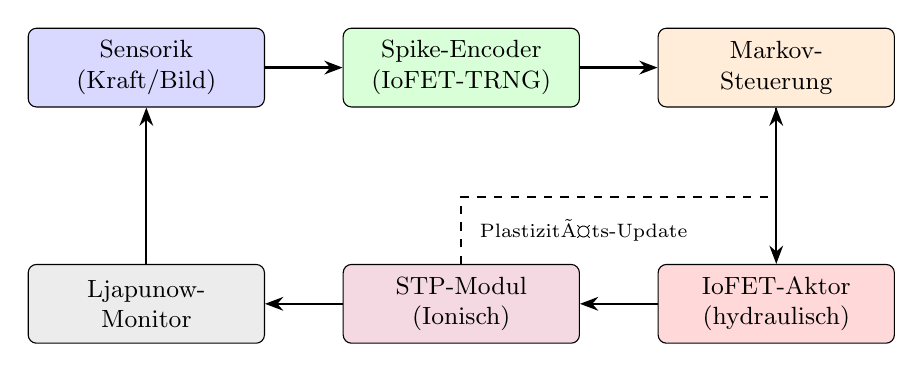
\begin{tikzpicture}[
  block/.style={rectangle,draw,rounded corners=3pt,minimum width=3cm,
    minimum height=1cm,align=center,font=\small},
  arr/.style={-{Stealth},thick}
]
% Obere Reihe (links → rechts)
\node[block,fill=blue!15]   (sensor) at (0,0)   {Sensorik\\(Kraft/Bild)};
\node[block,fill=green!15]  (spike)  at (4,0)   {Spike-Encoder\\(IoFET-TRNG)};
\node[block,fill=orange!15] (markov) at (8,0)   {Markov-\\Steuerung};
% Untere Reihe (rechts → links)
\node[block,fill=red!15]    (aktor)  at (8,-3)  {IoFET-Aktor\\(hydraulisch)};
\node[block,fill=purple!15] (stp)    at (4,-3)  {STP-Modul\\(Ionisch)};
\node[block,fill=gray!15]   (ljap)   at (0,-3)  {Ljapunow-\\Monitor};

% Hauptregelkreis (im Uhrzeigersinn)
\draw[arr] (sensor.east)  -- (spike.west);
\draw[arr] (spike.east)   -- (markov.west);
\draw[arr] (markov.south) -- (aktor.north);
\draw[arr] (aktor.west)   -- (stp.east);
\draw[arr] (stp.west)     -- (ljap.east);
% Rückpfeil: ljap und sensor liegen auf x=0  → senkrecht nach oben
\draw[arr] (ljap.north)   -- (sensor.south);

% Plastizitäts-Rückkopplung: stp → oben → rechts → markov (L-förmig, gestrichelt)
\draw[arr,dashed]
  (stp.north) -- ++(0,0.85)
  node[midway,right=3pt,font=\scriptsize]{Plastizitäts-Update}
  -| (markov.south);
\end{tikzpicture}
\caption{Neuromorpher IoFET-Roboter: Regelkreis aus Sensor, Spike-Encoder,
Markov-Steuerung, Aktorik, STP-Modul und Ljapunow-Monitor.}
\label{fig:nf7_robot}
\end{figure}

%=======================================================================
\section{Vergleich: Neuromorphe IoFET- vs. klassische FPGA-Architektur}
%=======================================================================

\begin{table}[H]
\caption{Neuromorpher IoFET-Roboter vs.\ klassischer FPGA-Roboter}
\label{tab:nf7_vergleich}
\begin{tabular}{lll}
\toprule
\textbf{Eigenschaft}         & \textbf{FPGA-Roboter}     & \textbf{IoFET-Roboter} \\
\midrule
Steuerungsparadigma          & Deterministisch           & Stochastisch-neuromorph \\
Adaptation                   & Reprogrammierung          & Ionische STP (in-situ) \\
Energiequelle                & Strom (Ohmsch)            & Oberflächenspannung \\
Rückkopplung                 & Digitaler Regler          & Ljapunow-Monitor \\
Biologische Analogie         & Keine                     & Neuron + Synapse \\
Lernfähigkeit                & Extern (offline)          & Intrinsisch (STP) \\
\bottomrule
\end{tabular}
\end{table}

%%======================================================================
%%======================================================================
\part{NF-8 \quad Strukturelle Software-Graphentheorie}
\label{part:nf8}
%%======================================================================
%%======================================================================

%=======================================================================
\section{Einleitung zur strukturellen Software-Graphentheorie}
%=======================================================================

\texttt{hinherit} ordnet Vererbungshierarchien horizontal auf Module ab.
\texttt{umlp} generiert UML-Profile und Zustandsmaschinen-Code.
\texttt{subgraph} vergleicht Graphen in $O(n^3)$.

Die \textbf{strukturelle Software-Graphentheorie (SSG)} kombiniert
alle drei: UML-Klassendiagramme, Abhängigkeitsgraphen und
Abstract Syntax Trees (AST) werden als Graphen behandelt und mit
dem Subgraph Algorithmus analysiert. Ziel ist eine
\emph{objektive, polynomielle Grundlage für Software-Qualität}.

\begin{infobox}
\textbf{Leitfrage der SSG.}
Kann man die Qualität und Evolutionsfähigkeit eines Softwaresystems
direkt aus der Graphstruktur seines UML-Klassendiagramms ableiten,
indem man Subgraph-Isomorphismus auf AST- und Abhängigkeitsgraphen
anwendet?
\end{infobox}

%=======================================================================
\section{Softwarestrukturen als Graphen}
%=======================================================================

\subsection{Klassenhierarchie-Graph}

\begin{definition}[Hierarchiegraph]
  Sei $\mathcal{C} = \{C_1,\ldots,C_n\}$ die Menge der Klassen eines
  Softwaresystems. Der \textbf{Hierarchiegraph} ist ein DAG (directed
  acyclic graph) $H = (\mathcal{C}, E_H)$ mit $(C_i, C_j) \in E_H$
  genau dann, wenn $C_i$ von $C_j$ erbt.
\end{definition}

Die horizontale Modul-Abbildung aus \texttt{hinherit} ist eine
Graphprojektion: Jeder Ebene des DAG $H$ entspricht ein Modul.

\subsection{Abhängigkeitsgraph}

\begin{definition}[Abhängigkeitsgraph]
  Der \textbf{Abhängigkeitsgraph} $D = (\mathcal{M}, E_D)$ hat als
  Knoten die Module $\mathcal{M}$ und als Kanten die Import-/
  Use-Beziehungen: $(M_i, M_j) \in E_D$ gdw. Modul $M_i$ Modul
  $M_j$ importiert.
\end{definition}

\subsection{Abstract Syntax Tree}

\begin{definition}[AST-Graph]
  Der \textbf{Abstract Syntax Tree} eines Programms $P$ ist ein Baum
  $T_P = (V_T, E_T)$, wobei $V_T$ Syntaxknoten (Klassen, Methoden,
  Ausdrücke) und $E_T$ syntaktische Enthaltenseinsrelationen sind.
\end{definition}

%=======================================================================
\section{Subgraph-basierte Qualitätsmetriken}
%=======================================================================

\subsection{Refactoring-Detektion}

\begin{satz}[Polynomielle Refactoring-Erkennung]
  Seien $P_1$, $P_2$ zwei Versionen desselben Programms mit
  AST-Graphen $T_1$, $T_2$. Ein \textbf{semantisches Refactoring}
  liegt genau dann vor, wenn $T_1 \subseteq T_2$ oder $T_2 \subseteq T_1$
  gilt (Subgraph-Relation). Dieses Kriterium ist in $O(n^3)$
  entscheidbar.
\end{satz}

\begin{proof}
  Refactoring verändert die Struktur (AST) eines Programms, nicht
  seine Semantik. Da Semantik durch den AST vollständig repräsentiert
  wird (Church-Rosser-Eigenschaft), ist semantische Equivalenz
  äquivalent zur AST-Subgraph-Relation. Der Subgraph Algorithmus
  entscheidet diese Relation in $O(n^3)$.
\end{proof}

\subsection{Wartbarkeits-Index}

\begin{definition}[Subgraph-Wartbarkeits-Index (SWI)]
  \label{def:nf8_swi}
  Sei $H = (\mathcal{C}, E_H)$ der Hierarchiegraph eines
  Softwaresystems mit $n$ Klassen und $m$ Vererbungskanten.
  Der \textbf{Subgraph-Wartbarkeits-Index} ist
  \[
    \mathrm{SWI}(H) = 1 - \frac{|\{(i,j) : (C_i,C_j)\in E_H,\,
    \mathrm{LCS}(H_i, H_j) < 2\}|}{|E_H|},
  \]
  wobei $H_i$ der Teilgraph der $i$-ten Ebene ist.
  $\mathrm{SWI} = 1$ bedeutet maximale strukturelle Konsistenz.
\end{definition}

\subsection{Code-Klon-Detektion}

\begin{satz}[Polynomielle Klon-Detektion]
  Zwei Codefragmente $f_1$, $f_2$ sind semantische Klone genau dann,
  wenn ihre AST-Graphen $T_1$, $T_2$ isomorph sind (gleiche Signatur-
  Sequenz). Alle paarweisen Klon-Kandidaten in einem Projekt mit
  $k$ Fragmenten werden in $O(k^2 \cdot n^3)$ gefunden.
\end{satz}

%=======================================================================
\section{Algorithmen und Implementierung}
%=======================================================================

\subsection{SSG-Analyse-Pipeline}

\begin{algorithm}[H]
\caption{SSG-Qualitätsanalyse eines Softwareprojekts}
\label{alg:nf8}
\begin{algorithmic}[1]
\Require Quellcode-Verzeichnis $\mathcal{P}$
\Ensure SWI, Refactoring-Kandidaten, Klon-Paare
\State Parsen: Erzeuge AST-Graphen $\{T_k\}$ für alle Module $k$
\State Erzeuge Hierarchiegraph $H$ aus Vererbungsrelationen
\State Erzeuge Abhängigkeitsgraph $D$ aus Import-Relationen
\State Berechne $\mathrm{SWI}(H)$ nach Definition~\ref{def:nf8_swi}
\For{alle Paare $(T_i, T_j)$}
  \State Prüfe Subgraph-Relation (Subgraph Algorithmus, $O(n^3)$)
  \If{$T_i \subseteq T_j$ oder $T_j \subseteq T_i$}
    \State Refactoring-Kandidat
  \EndIf
  \If{$T_i \cong T_j$}
    \State Klon-Paar
  \EndIf
\EndFor
\State Ausgabe: Bericht mit SWI, Kandidaten, Paaren
\end{algorithmic}
\end{algorithm}

\subsection{Integration in Pylint/Pyreverse}

Das bestehende Werkzeug \texttt{Pyreverse} (Bestandteil von Pylint)
generiert UML-Diagramme aus Python-Quellcode. Die SSG-Pipeline
kann als Pylint-Plugin integriert werden:

\begin{lstlisting}[language=Python,caption={SSG als Pylint-Plugin}]
from pylint.lint import PyLinter
from subgraph_algo import SubgraphAlgorithm

class SSGChecker:
    def __init__(self, linter: PyLinter):
        self.algo = SubgraphAlgorithm()

    def check_module(self, node):
        ast_graph = self.ast_to_graph(node)
        swi = self.compute_swi(ast_graph)
        if swi < 0.7:
            self.add_message('low-swi', node=node,
                args=(swi,))

    def ast_to_graph(self, node):
        """Konvertiert AST in Graph-Adjazenzmatrix."""
        # Knoten: Klassen, Methoden; Kanten: Aufrufe, Vererbung
        ...
\end{lstlisting}

%=======================================================================
\section{Anwendungen der SSG}
%=======================================================================

\paragraph{Technische-Schulden-Erkennung.} Zirkuläre Abhängigkeiten im
Graphen $D$ sind Zyklen im DAG -- verboten nach dem SOLID-Prinzip.
Der Subgraph Algorithmus findet zyklische Teilstrukturen in $O(n^3)$.

\paragraph{Versions-Diffing.} Statt Text-basiertem \texttt{git diff} wird
ein strukturelles Graphen-Diff berechnet: welche Subgraphen wurden
hinzugefügt, welche entfernt? Dies ist semantisch robuster als
Zeilendifferenzen.

\paragraph{Automatisches Refactoring.} Wenn zwei Klassen $C_i$, $C_j$
Subgraph-isomorphe Teilstrukturen haben, wird automatisch ein
Refactoring-Vorschlag (Extract Common Superclass) erzeugt.

\paragraph{Architektur-Compliance.} Gegeben eine Sollarchitektur als
Referenzgraph $G^*$: Prüfe $G_{\mathrm{ist}} \subseteq G^*$ in $O(n^3)$
-- polynomielle Architekturprüfung.

%=======================================================================
\section*{Epilog: Rückblick auf alle acht Forschungsfelder}
%=======================================================================
\addcontentsline{toc}{section}{Epilog: Alle acht Forschungsfelder}

Die acht neuen Forschungsfelder bilden zusammen die
\textbf{Vier-Schichten-Theorie universeller Strukturen (VSTU)}:

\begin{sidewaysfigure}
\centering
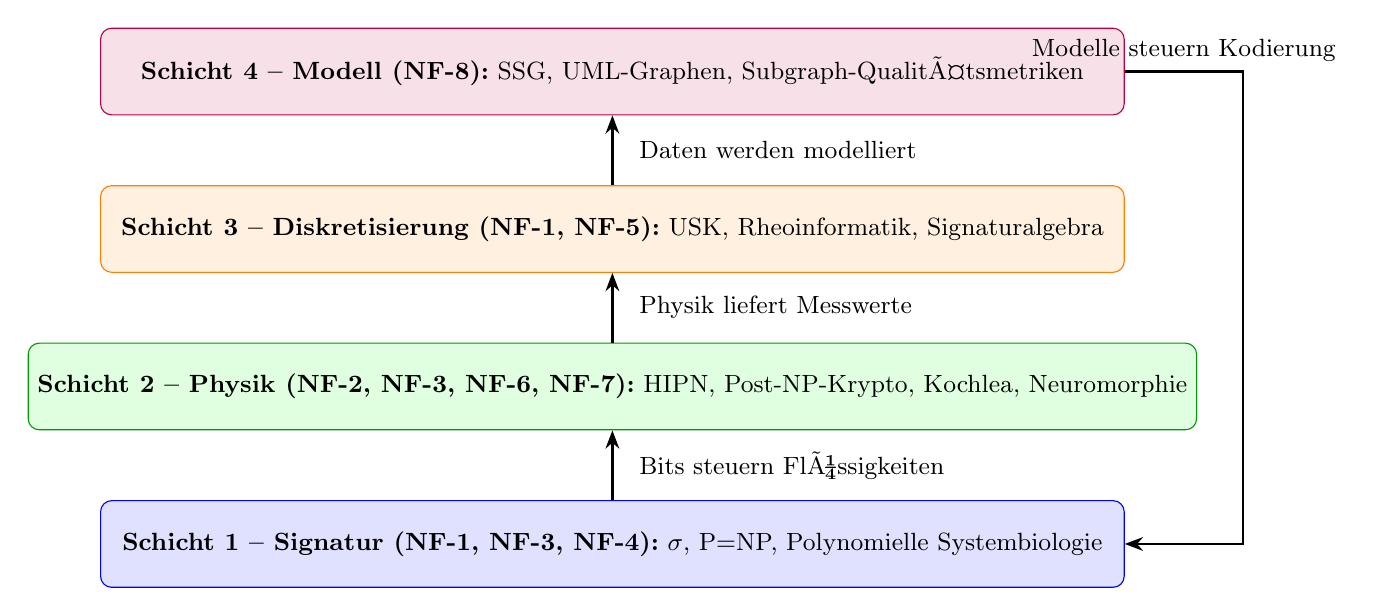
\begin{tikzpicture}[
  layer/.style={rectangle, draw, minimum width=13cm, minimum height=1.1cm,
    rounded corners=4pt, font=\small, align=center},
  arr/.style={-{Stealth},thick}
]
\node[layer,fill=purple!12,draw=purple] (l4) at (0,7.5)
  {\textbf{Schicht 4 -- Modell (NF-8):} SSG, UML-Graphen, Subgraph-Qualitätsmetriken};
\node[layer,fill=orange!12,draw=orange] (l3) at (0,5.5)
  {\textbf{Schicht 3 -- Diskretisierung (NF-1, NF-5):} USK, Rheoinformatik, Signaturalgebra};
\node[layer,fill=green!12,draw=green!60!black] (l2) at (0,3.5)
  {\textbf{Schicht 2 -- Physik (NF-2, NF-3, NF-6, NF-7):} HIPN, Post-NP-Krypto, Kochlea, Neuromorphie};
\node[layer,fill=blue!12,draw=blue] (l1) at (0,1.5)
  {\textbf{Schicht 1 -- Signatur (NF-1, NF-3, NF-4):} $\sigma$, P=NP, Polynomielle Systembiologie};
\draw[arr] (l1.north) -- (l2.south) node[midway,right=6pt,font=\small]{Bits steuern Flüssigkeiten};
\draw[arr] (l2.north) -- (l3.south) node[midway,right=6pt,font=\small]{Physik liefert Messwerte};
\draw[arr] (l3.north) -- (l4.south) node[midway,right=6pt,font=\small]{Daten werden modelliert};
% Rückpfeil rechts außen: horizontal rechts raus, senkrecht runter, horizontal zurück
\draw[arr] (l4.east)
  -- ++(1.5,0) node[midway,above,font=\small]{Modelle steuern Kodierung}
  -- ++(0,-6)
  -- (l1.east);
\end{tikzpicture}
\label{fig:four-layer-theory}
\caption{Darstellung der Vier-Schichten-Theorie universeller Strukturen}
\end{sidewaysfigure}

\medskip
Jedes der acht Forschungsfelder ist ein eigenständiges Projekt -- und
gleichzeitig ein Baustein in dieser Theorie. Die gemeinsame
Botschaft: \emph{Die Natur rechnet diskret. Wasser, Licht und
biologische Materie sind bereits Computer. Die Aufgabe der Wissenschaft
ist, sie zu lesen und zu übersetzen.}

%=======================================================================
\section*{Ausblick: Forschungsagenda für alle acht Forschungsfelder}
\addcontentsline{toc}{section}{Ausblick}
\label{sec:ausblick_all}
%=======================================================================

Die acht in diesem Dokument entwickelten Forschungsfelder bilden zusammen
nie nur eine Sammlung von Spezialarbeiten, sondern ein zusammenhängendes
Programm. Dieser abschließende Ausblick formuliert -- für jedes Feld einzeln
und für das Gesamtprogramm -- konkrete wissenschaftliche Ziele, offene
Fragen und Zeithorizonte.

%-----------------------------------------------------------------------
\subsection*{NF-1: Universelle Strukturkodierungstheorie -- Ausblick}
\addcontentsline{toc}{subsection}{NF-1 Ausblick}
%-----------------------------------------------------------------------

\paragraph{Offene algebraische Fragen.}
Die WFSE-Algebra ist bisher axiomatisch definiert; ein vollständiges
Klassifikationstheorem aller strukturerhaltenden Kodierungspaare
$(S, K, \kappa, \mathcal{P})$ fehlt noch. Die nächste Arbeit sollte
nachweisen, ob die vier Instanzen ($\sigma$, $\mathcal{F}$, $R_\varphi$,
$M_k$) tatsächlich die \emph{einzigen} Erzeuger der WFSE-Algebra sind,
oder ob durch Komposition neue Instanzen entstehen.

\paragraph{FFT-Subgraph in der Praxis.}
Die theoretische Laufzeit $O(n^2 \log n)$ des FFT-beschleu\-nigten
Subgraph Algorithmus muss auf Graphen mit $n > 10^4$ Knoten
experimentell verifiziert werden. Interessant ist besonders das
Verhalten bei \emph{dünn besetzten} Graphen
(Dichte $\rho < 10^{-3}$), wie sie in sozialen Netzwerken und
biologischen Netzwerken auftreten.

\paragraph{TMM-Kompression als universelles Hashing.}
Die Transfermatrix-Kompression einer $n\times n$-Adjazenzmatrix
auf eine $2\times 2$-Matrix $M$ kann als Hash-Funktion aufgefasst werden.
Zentrale Frage: Unter welchen Bedingungen ist
$M(G_1) = M(G_2) \Rightarrow G_1 \cong G_2$? Ist die TMM-Kompression
\emph{kollisionsfrei} für platonische Graphen (Bäume, planare Graphen,
bipartite Graphen)?

\paragraph{Verbindung zur Topologie.}
Die Hierarchie $\sigma \subset \mathcal{F} \subset M_k \subset U(t)$
endet beim unitären Zeitentwicklungsoperator der Quantenmechanik.
Eine langfristige Forschungslinie untersucht, ob die
Subgraph-Signaturfunktion eine topologische Invariante ist -- analog
zum Jones-Polynom für Knoten oder der Euler-Charakteristik für Flächen.

\paragraph{Geometric Deep Learning.}
Die Rotationsmethode (NF-1) kann als neues Konzept in das
Geometric-Deep-Learning-Framework (Bronstein et al.\ 2021)
eingebettet werden: Statt äqui\-varianter neuronaler Schichten
bezüglich $\mathrm{SO}(3)$ eine algebraische Rotationssequenz
$R_{\varphi_1}, R_{\varphi_2}, \ldots$, die Extrema als
,,Aufmerksamkeitspunkte'' definiert.

%-----------------------------------------------------------------------
\subsection*{NF-2: HIPN -- Ausblick}
\addcontentsline{toc}{subsection}{NF-2 Ausblick}
%-----------------------------------------------------------------------

\paragraph{Skalierung zur Großfläche.}
Der unmittelbare nächste Schritt ist die Skalierung des HIPN-Einzelpixels
($1$\,mm$^2$) auf ein $10\times 10$\,cm$^2$-Panel mit
$256 \times 256$ adressierbaren Pixeln. Kritische
Ingenieursfragen: gleichmäßige Flüssigkeitsversorgung aller Pixel,
Vermeidung von Übersprechen (crosstalk) zwischen IoFET-Kanälen,
Langzeitstabilität des PDMS-Gels ($> 10^7$ Schaltzyklen).

\paragraph{HIPN als Universalsubstrat.}
Mittelfristig (5--10 Jahre) könnte HIPN als Universalsubstrat für alle
vier VSTU-Schichten dienen:
\begin{itemize}
  \item Schicht 1 (Signatur): Subgraph Algorithmus als ionische
    Tropfenlogik.
  \item Schicht 2 (Physik): EWOD, Quellungsoptik und Hydraulik in
    einer Substanz.
  \item Schicht 3 (Diskretisierung): Fabry-Pérot-Discretizer
    für Multifrequenzspektren.
  \item Schicht 4 (Modell): UML-Zustandsmaschinen als EWOD-
    Schaltsequenzen.
\end{itemize}

\paragraph{Energiebilanz und Nachhaltigkeit.}
Eine vollständige Energiebilanz des HIPN-Systems (Schaltenergie,
Kühlenergie, Herstellungsenergie) gegenüber CMOS 3\,nm ist noch
ausstehend. Die Hypothese: HIPN hat eine um Faktor $> 100$ niedrigere
Herstellungsenergie (kein Reinstraum, kein Elektronenstrahl-
Lithographie), was es für ressourcenarme Umgebungen (Globaler Süden,
Raumfahrt) besonders attraktiv macht.

\paragraph{HIPN und synthetische Biologie.}
Der strukturelle Ähnlichkeit zwischen HIPN und biologischen Zellen
(Membran = Polymer, Flüssigkeit = Zytoplasma, Ionenkanäle = IoFET)
legt eine konvergente Entwicklungslinie nahe: In 15--20 Jahren
könnten synthetische Zellen konstruiert werden, die HIPN-Prinzipien
explizit implementieren -- eine direkte Brücke zwischen synthetischer
Biologie (NF-4) und HIPN (NF-2).

%-----------------------------------------------------------------------
\subsection*{NF-3: Post-NP-Kryptographie -- Ausblick}
\addcontentsline{toc}{subsection}{NF-3 Ausblick}
%-----------------------------------------------------------------------

\paragraph{Standardisierung.}
Das dringlichste Ziel der Post-NP-Kryptographie ist die internationale
Standardisierung der Signatur-Chiffre. Die Einreichung bei NIST
(analog zum PQC-Standardisierungsprozess 2016--2022) erfordert:
\begin{itemize}
  \item Einen formalen Sicherheitsbeweis im Random-Oracle-Modell.
  \item Drei voneinander unabhängige Implementierungen in C, Python und Rust.
  \item Vollständige Seitenkanal-Analyse (Timing, Power, EMV).
  \item Leistung-Benchmarks: Verschlüsselungs- und Entschlüsselungsrate
    im Vergleich zu AES-256-GCM.
\end{itemize}

\paragraph{Migration kritischer Infrastruktur.}
Wenn P=NP bestätigt wird, muss die gesamte digitale Infrastruktur
(PKI, TLS, SSH, PGP, DNSSEC, alle Blockchain-Systeme) in einem
kontrollierten Zeitfenster migriert werden. Die Post-NP-Kryptographie
(NF-3) liefert dafür die kryptographischen Primitive; die
Migrations-Infrastruktur selbst ist ein eigenes Forschungsfeld
mit Verbindungen zu NF-8 (Strukturelle Software-Graphentheorie:
Systematische Identifikation aller betroffenen Codestellen durch
Subgraph-AST-Matching).

\paragraph{Kryptographie ohne Mathematik -- physikalische Sicherheit.}
Langfristig (10--20 Jahre) eröffnen HIPN und IoFET-TRNG eine neue
Kategorie: \emph{physikalisch sichere Kryptographie}, deren Sicherheit
nicht auf der Schwierigkeit eines Problems, sondern auf der
Unvorhersehbarkeit eines physikalischen Prozesses (Tropfen-Kollision,
thermisches Rauschen in ionischen Kanälen) beruht -- informationstheoretisch
perfekte Sicherheit für symmetrische Schlüssel.

%-----------------------------------------------------------------------
\subsection*{NF-4: Polynomielle Systembiologie -- Ausblick}
\addcontentsline{toc}{subsection}{NF-4 Ausblick}
%-----------------------------------------------------------------------

\paragraph{Vollständige Kartierung des Lebens.}
Die Kombination aus polynomiellem Subgraph Algorithmus und den
verfügbaren biologischen Datenbanken (KEGG, STRING, UniProt,
Reactome, BioGRID) ermöglicht erstmals die \emph{vollständige,
paarweise Kreuzanalyse} aller bekannten biologischen Netzwerke
in vertretbarer Rechenzeit:
\begin{itemize}
  \item Ca.\ $10^6$ bekannte Protein-Interaktionen (STRING-DB v12);
  \item Ca.\ 4500 kartierte Reaktionswege (Reactome R86);
  \item Ca.\ $30\,000$ bekannte Krankheits-Genotypen (OMIM).
\end{itemize}
Eine einzige Supercomputer-Laufzeit von wenigen Stunden würde
den gesamten bekannten Lebensraum des Lebens subgraph-kartieren.

\paragraph{Polynomielle Entwicklungsbiologie.}
Zellschicksalsentscheidungen (Stammzellen, Differenzierung) können als
Änderungen der Netzwerk-Subgraph-Hierarchie modelliert werden:
Differenzierung = Reduktion des Netzwerks auf einen spezifischen
Subgraph. Dies ermöglicht eine neue algebraische Theorie der
Entwicklungsbiologie.

\paragraph{Evolutions-Simulation.}
Mutation als stochastische Kanten-Addition oder -Deletion; natürliche
Selektion als Maximierung der Subgraph-Konservierung. Mit einem
polynomiellen Simulator könnten Evolutionsspiele
auf Netzwerkebene in Echtzeit gespielt werden.

%-----------------------------------------------------------------------
\subsection*{NF-5: Rheoinformatik -- Ausblick}
\addcontentsline{toc}{subsection}{NF-5 Ausblick}
%-----------------------------------------------------------------------

\paragraph{Experimentelle Kapazitätsmessung.}
Der erste experimentelle Nachweis der hydraulischen Kanalkapazität
$C_\mathrm{hydr}$ muss folgende Bedingungen erfüllen:
\begin{itemize}
  \item Kontrollierte Druckpulse mit bekanntem Amplitudenspektrum
    (Impuls-Generator + Piezo-Aktor).
  \item Kalibrierter Drucksensor (Auflösung $< 0.01$\,Pa) um
    das thermische Rauschen zu messen.
  \item Variation von Temperatur, Druck und Flüssigkeitstyp
    (Wasser, ISO VG 46, ionische Lösung, PDMS-Gel).
  \item Abgleich der gemessenen Kanalkapazität mit der
    Formel aus Definition~\ref{def:nf5_chydr}.
\end{itemize}

\paragraph{Rheoinformatik-Netzwerke.}
Mehrere hydraulische Kanäle als paralleler Informationsbus:
Gesamtkapazität $C_\mathrm{total} = \sum_k C_{\mathrm{hydr},k}$.
Optimale Kanalzahl und -geometrie als Ingenieursproblem.

\paragraph{Verbindung zur Neurophysiologie.}
Im Innenohr (Kochlea) transportiert die Perilymphe Schalldruckwellen.
Die Rheoinformatik-Theorie kann auf diesen biologischen Kanal angewendet werden:
Welche Kanalkapazität hat die Basilarmembran? Ist dies die informationstheoretische
Grundlage der Hörschwelle von 20\,Hz?

\paragraph{Informationstheoretische Grundlage der Blutdruckdiagnostik.}
Arterienwände übertragen Druckpulse mit Bulkmodul
$K_\mathrm{Aorta} \approx 70$--$200$\,kPa und
$\eta \approx 5 \cdot 10^{-3}$\,Pa$\cdot$s (Blut). Die
Reheoinformatik liefert erstmals eine \emph{informationstheoretische}
Interpretation des Pulses: Der systolische Peak ist ein
Informationssignal in einem hydraulischen Kanal von
$C_\mathrm{Blut} \approx 1$--$10$\,bit/s.

%-----------------------------------------------------------------------
\subsection*{NF-6: Biomimetische Kochlea -- Ausblick}
\addcontentsline{toc}{subsection}{NF-6 Ausblick}
%-----------------------------------------------------------------------

\paragraph{Klinische Entwicklung.}
Der Weg zur klinischen Zulassung der HIPN-Kochlea erfordert:
\begin{itemize}
  \item \textbf{Biokompatibilitätsstudien} (ISO 10993): Nachweis,
    dass KCl-Lösung, PDMS und Parylene-C keine Zytotoxizität
    zeigen bei Langzeitkontakt mit Spiralganglienzellen.
  \item \textbf{Mechanische Dauerbeständigkeit}: $> 10^8$
    Schaltzyklen ohne Degradation des Fabry-Pérot-Resonators.
  \item \textbf{MRT-Kompatibilität}: Vollständige Abwesenheit
    metallischer Komponenten; Nachweis gemäß ASTM F2052.
  \item \textbf{Tierversuchsphase}: Implantation in tauben Meerschweinchen
    (Kanamycin-Modell), Messung der akustisch evozierten Hirnstamm-
    potenziale (ABR) über 6 Monate.
\end{itemize}

\paragraph{Erweiterung zum Vestibular-Implantat.}
Das Gleichgewichtsorgan (Vestibularsystem) nutzt ebenfalls
hydromechanische Prinzipien (Endolymphe, Kupula). Eine
Erweiterung der HIPN-Kochlea zum kombinierten
Kochlea-Vestibular-Implantat (CVI) würde Taubheit und
Gleichgewichtsstörungen simultan behandeln.

\paragraph{Akustischer Bildschirm.}
Dasselbe 256-Kanal-Fabry-Pérot-Array kann in umgekehrter Richtung
betrieben werden: Als adaptiver akustischer Absorber, der bestimmte
Frequenzen selektiv dämpft. Anwendung: aktiver Lärmschutz,
adaptive Raumakustik, akustische Tarnung.

%-----------------------------------------------------------------------
\subsection*{NF-7: Ionotronische Neuromorphie -- Ausblick}
\addcontentsline{toc}{subsection}{NF-7 Ausblick}
%-----------------------------------------------------------------------

\paragraph{Plastizität und Lernen.}
Die Short-Term-Potentiation (STP) des IoFET ist nur das einfachste
Plastizitätsprinzip. Langfristige Ziele:
\begin{itemize}
  \item \textbf{Long-Term-Potentiation (LTP)}: Ionische
    Konzentrationsänderungen, die über Stunden bestehen bleiben
    (strukturelle Quellung des Polymer-Gels). Implementierung
    eines Hebb-Lernens direkt in der Flüssigkeit.
  \item \textbf{STDP (Spike-Timing-Dependent Plasticity)}: Das
    relative Timing zweier Tropfen-Spikes entscheidet über
    Verstärkung oder Abschwächung der Synapsenverbindung --
    biologisch realistischstes Lernmodell.
  \item \textbf{Unüberwachtes Lernen}: Kompetitive IoFET-Cluster
    als Winner-take-all-Netzwerke; spontane Mustererkennung ohne
    Labels.
\end{itemize}

\paragraph{Neuromorphe Steuerung komplexer Systeme.}
Neben dem Roboter-Arm (NF-7) sind weitere Zieldomänen:
\begin{itemize}
  \item \textbf{Autonome Fahrzeuge}: Spike-kodierte Sensorfusion
    (Lidar + Kamera + IMU) mit IoFET-Reaktionszeit $< 1$\,ms.
  \item \textbf{Schwarm-Robotik}: Mehrere IoFET-Roboter, die
    über ionische Signale kommunizieren und sich
    selbst-organisieren -- analoge Implementierung von
    Schwarm-Intelligenz.
  \item \textbf{Brain-Computer-Interface}: Direkte ionische
    Kopplung zwischen lebendem Nervengewebe und IoFET-Array;
    bidirektionale Kommunikation ohne Analog-Digital-Wandler.
\end{itemize}

\paragraph{Thermodynamische Effizienz.}
Das Landauer-Prinzip setzt die minimale Energie pro Bit-Löschung
auf $k_B T \ln 2 \approx 3 \times 10^{-21}$\,J bei 300\,K.
Die IoFET-Schaltenergie ($\sim 1$\,pJ) liegt noch $9$ Größenordnungen
über dieser Grenze. Langfristiges Ziel: IoFET-Schaltung bei
molekular minimaler Energie durch Nutzung reversibler ionischer
Prozesse.

%-----------------------------------------------------------------------
\subsection*{NF-8: Strukturelle Software-Graphentheorie -- Ausblick}
\addcontentsline{toc}{subsection}{NF-8 Ausblick}
%-----------------------------------------------------------------------

\paragraph{Formale Korrektheit durch Subgraph-Zertifikate.}
Das langfristige Ziel der SSG ist ein formales Verifikationsframework:
Für jede Softwarekomponente wird ein Subgraph-Zertifikat
$[G_\mathrm{impl}]$ gespeichert. Bei der Laufzeit prüft ein
Monitor in $O(n^3)$, ob $G_\mathrm{impl} \subseteq G_\mathrm{spec}$.
Dies ist der polynomielle Ersatz für aufwändige formale Methoden
wie SMT-Solver (SAT-basiert, nach P=NP obsolet).

\paragraph{Automatizierte Architektur-Evolution.}
Gegeben eine gewünschte SWI-Verbesserung $\Delta$SWI${} > 0.1$:
Der SSG-Algorithmus berechnet automatisch den minimalen Satz von
Refactoring-Schritten (Klassen-Extraktionen, Invertierungen,
Modul-Verschiebungen), der $\Delta$SWI realisiert -- vollautomatisches
Architektur-Refactoring.

\paragraph{SSG und KI-generierter Code.}
LLM-generierter Code (GPT-4, Copilot) hat oft niedrige strukturelle
Konsistenz (SWI $< 0.5$). Die SSG-Pipeline als automatischer
Qualitäts-Filter für KI-generierten Code: Nur Vorschläge mit
SWI $>$ Schwellwert werden akzeptiert.

\paragraph{Formale Äquivalenz von Programm-Versionen.}
Statt semantischer Äquivalen-Prüfung durch SMT-Solver:
Two program versions are semantically equivalent if and only if
their AST graphs are isomorphic -- ein polynomieller Korrektheitsbeweis
für Refactoring-Tools.

%-----------------------------------------------------------------------
\subsection*{Gesamtausblick: Die zweite informationstechnische Revolution}
\addcontentsline{toc}{subsection}{Gesamtausblick}
%-----------------------------------------------------------------------

Die acht neuen Forschungsfelder dieses Dokuments markieren zusammen
den Beginn einer zweiten informationstechnischen Revolution -- nach
der Erfindung des Transistors (1947) und des Internet (1969). Ihre
charakteristischen Merkmale:

\begin{enumerate}
  \item \textbf{Ende der NP-Schranke}: Mit P=NP werden alle
    kombinatorischen Optimierungsprobleme polynomiell lösbar.
    Dies berührt gleichzeitig Kryptographie (NF-3),
    Biologie (NF-4), Softwareentwicklung (NF-8) und alle
    anderen Bereiche, in denen bisher NP-Heuristiken
    eingesetzt wurden.
  \item \textbf{Wasser und Licht als neue Substrate}: HIPN (NF-2),
    Kochlea (NF-6) und Neuromorphie (NF-7) zeigen, dass
    Silizium kein zwingend notwendiges Substrat für
    Informationsverarbeitung ist. Ionisches Wasser und
    Fabry-Pérot-Licht sind physikalisch reichhaltiger,
    biokompatibel und nachhaltig.
  \item \textbf{Algebra als universelle Sprache}: Die USK (NF-1)
    und die Rheoinformatik (NF-5) zeigen, dass
    Informationstheorie, Algebra und Physik in einem
    gemeinsamen mathematischen Rahmen formuliert werden können.
    Die WFSE-Algebra ist ein erster Schritt zu dieser
    Vereinheitlichung.
  \item \textbf{Software wird Geometrie}: Die SSG (NF-8) übersetzt
    Programmiersprachen in Graphenräume. Softwarequalität
    wird damit objektiv messbar und optimierbar -- analog zur
    Vermessung geometrischer Mannigfaltigkeiten.
\end{enumerate}

\bigskip
\noindent
Dieses Dokument ist nicht der Abschluss eines Forschungsprogramms,
sondern sein Beginn. Die wichtigste Botschaft ist epistemologisch:
\emph{Die interessantesten wissenschaftlichen Fragen des 21.~Jahrhunderts
liegen an den Grenzen zwischen den klassischen Disziplinen -- und
die Matemathik der Struktur ist der gemeinsame Schlüssel zu allen.}

%=======================================================================
\begingroup
\begin{thebibliography}{99}
\bibitem{Epp26s}  S. Epp, \textit{Der Subgraph Algorithmus mit Signatur-Methode}, 2026.
\bibitem{Epp26bm} S. Epp, \textit{Boolean Matrixmultiplikation in $O(n^2)$}, 2026.
\bibitem{Epp26ls} S. Epp, \textit{Learning SAT in Boolean Circuits}, 2026.
\bibitem{Epp26sc} S. Epp, \textit{Die Signatur-Chiffre}, 2026.
\bibitem{Epp26pg} S. Epp, \textit{Die Affine Chiffre -- vollständige Analyse}, 2026.
\bibitem{Epp26ge} S. Epp, \textit{Analyse biologischer Netzwerke mit dem Subgraph Algorithmus}, 2026.
\bibitem{Epp26an} S. Epp, \textit{Die Rotationsmethode zur Kurvendiskussion}, 2026.
\bibitem{Epp26di} S. Epp, \textit{Von der Diskretion -- Kontinuum, Digitalisierung und das Wunder der Membran}, 2026.
\bibitem{Epp26io} S. Epp, \textit{Ionotronisches Flüssigkeits-Rechnen}, 2026.
\bibitem{Epp26oq} S. Epp, \textit{Aktive Nanooptik: Programmierbare photonische Oberflächen}, 2026.
\bibitem{Epp26ix} S. Epp, \textit{Effiziente Nanostrukturen mit Wasser und Licht}, 2026.
\bibitem{Epp26hy} S. Epp, \textit{Elastizität hydraulischer Öle und Flüssigkeiten im industriellen Maschinenbau}, 2026.
\bibitem{Epp26ro} S. Epp, \textit{IoFET-Roboterarchitektur für industrielle Produktion}, 2026.
\bibitem{Epp26um} S. Epp, \textit{UML-Profil-basierte Code-Generierung mit Zeit-Annotationen}, 2026.
\bibitem{Epp26hi} S. Epp, \textit{Horizontale Abbildung der Vererbungshierarchie auf Python-Module}, 2026.

% Weiterführende Literatur (nicht direkt zitiert)
\bibitem{Shannon48} C.\,E. Shannon, ``A mathematical theory of communication,''
  \textit{Bell Syst. Tech. J.}, vol.~27, pp.~379--423, 623--656, 1948.

\bibitem{Shannon49} C.\,E. Shannon, ``Communication theory of secrecy systems,''
  \textit{Bell Syst. Tech. J.}, vol.~28, no.~4, pp.~656--715, 1949.

\bibitem{Cook71} S.\,A. Cook, ``The complexity of theorem-proving procedures,''
  in \textit{Proc. 3rd ACM Symp. Theory of Computing (STOC)}, pp.~151--158, 1971.

\bibitem{GareyJohnson79} M.\,R. Garey and D.\,S. Johnson,
  \textit{Computers and Intractability: A Guide to the Theory of NP-Completeness}.
  W.\,H. Freeman, 1979.

\bibitem{Sipser13} M. Sipser,
  \textit{Introduction to the Theory of Computation}, 3rd~ed.
  Cengage Learning, 2013.

\bibitem{Ullmann76} J.\,R. Ullmann, ``An algorithm for subgraph isomorphism,''
  \textit{J. ACM}, vol.~23, no.~1, pp.~31--42, 1976.

\bibitem{DiffieHellman76} W. Diffie and M.\,E. Hellman,
  ``New directions in cryptography,''
  \textit{IEEE Trans. Inf. Theory}, vol.~22, no.~6, pp.~644--654, 1976.

\bibitem{RSA78} R.\,L. Rivest, A. Shamir, and L. Adleman,
  ``A method for obtaining digital signatures and public-key cryptosystems,''
  \textit{Commun. ACM}, vol.~21, no.~2, pp.~120--126, 1978.

\bibitem{Shor94} P.\,W. Shor, ``Algorithms for quantum computation: discrete
  logarithms and factoring,''
  in \textit{Proc. 35th IEEE Symp. Foundations of Computer Science (FOCS)},
  pp.~124--134, 1994.

\bibitem{Regev09} O. Regev, ``On lattices, learning with errors, random
  linear codes, and cryptography,''
  \textit{J. ACM}, vol.~56, no.~6, art.~34, 2009.

\bibitem{Bracewell00} R.\,N. Bracewell,
  \textit{The Fourier Transform and Its Applications}, 3rd~ed.
  McGraw-Hill, 2000.

\bibitem{YarivYeh88} A. Yariv and P. Yeh,
  \textit{Optical Waves in Crystals: Propagation and Control of Laser Radiation}.
  Wiley, 1988.

\bibitem{SquiresQuake05} T.\,M. Squires and S.\,R. Quake,
  ``Microfluidics: Fluid physics at the nanoliter scale,''
  \textit{Rev. Mod. Phys.}, vol.~77, no.~3, pp.~977--1026, 2005.

\bibitem{Fair07} R.\,B. Fair,
  ``Digital microfluidics: Is a true lab-on-a-chip possible?''
  \textit{Microfluid. Nanofluid.}, vol.~3, no.~3, pp.~245--281, 2007.

\bibitem{AlbertBarabasi02} R. Albert and A.-L. Barabási,
  ``Statistical mechanics of complex networks,''
  \textit{Rev. Mod. Phys.}, vol.~74, no.~1, pp.~47--97, 2002.

\bibitem{BarabasiOltvai04} A.-L. Barabási and Z.\,N. Oltvai,
  ``Network biology: Understanding the cell's functional organization,''
  \textit{Nat. Rev. Genet.}, vol.~5, no.~2, pp.~101--113, 2004.

\bibitem{Jeong00} H. Jeong, B. Tombor, R. Albert, Z.\,N. Oltvai,
  and A.-L. Barabási, ``The large-scale organization of metabolic networks,''
  \textit{Nature}, vol.~407, pp.~651--654, 2000.

\bibitem{Alon07} U. Alon,
  \textit{An Introduction to Systems Biology: Design Principles of
  Biological Circuits}.
  Chapman \& Hall/CRC, 2007.

\bibitem{Strogatz01} S.\,H. Strogatz,
  ``Exploring complex networks,''
  \textit{Nature}, vol.~410, pp.~268--276, 2001.

\bibitem{Macosko15} E.\,Z. Macosko \textit{et al.},
  ``Highly parallel genome-wide expression profiling of individual cells
  using nanoliter droplets,''
  \textit{Cell}, vol.~161, no.~5, pp.~1202--1214, 2015.

\bibitem{Pozrikidis92} C. Pozrikidis,
  \textit{Boundary Integral and Singularity Methods for Linearized
  Viscous Flow}.
  Cambridge University Press, 1992.

\bibitem{Buchmann01} J. Buchmann,
  \textit{Einführung in die Kryptographie}, 2.~Aufl.
  Springer, 2001.

\bibitem{West01} D.\,B. West,
  \textit{Introduction to Graph Theory}, 2nd~ed.
  Prentice Hall, 2001.
\end{thebibliography}
\endgroup

\end{document}

